%----------------------------------------------------------------------------------------
%	PACKAGES AND OTHER DOCUMENT CONFIGURATIONS
%----------------------------------------------------------------------------------------
\documentclass[12pt, letter, oneside]{Thesis} % Paper size, default font size and one-sided paper
%\graphicspath{{Pictures/}} % Specifies the directory where pictures are stored
\usepackage{hyperref} % For internal referencing
\usepackage{lipsum} % For generating fill text for trouble-shooting LaTex
\usepackage{setspace} % For picking line spacing *within* sections
\usepackage{parskip} % For changing spacing between heads, lets me use linebreaks for spacing between paragraphs
\usepackage{float}% For Figures
	\floatstyle{plain}
	\restylefloat{figure}
	\usepackage{rotating} % For rotating figures ±90˚ use \begin{sidewaysfigure}	
%% Pick my Font
	% For Palatino
	%\usepackage[sc]{mathpazo}
	%	\linespread{1.05} % Palatino needs more leading (space between lines)
	% For Ariel
	\usepackage{helvet}
	\renewcommand{\familydefault}{\sfdefault}

% Center the Chapter and heading titles 
% http://tex.stackexchange.com/questions/23858/center-chapter-book-class
	\usepackage{titlesec}
	\titleformat{\chapter}[display]
	{\normalfont\huge\bfseries\centering}{\chaptertitlename\ \thechapter}{20pt}{\Huge}

\usepackage[T1]{fontenc} 
\usepackage{flexisym} % Lets me use prime symbols
\usepackage{gensymb} % For degree '\degree'

% For Referencing
\usepackage[square, comma, sort&compress]{natbib} 
	\setlength{\bibsep}{0.0pt} % Reduce size of bibliography
	% Use the natbib reference package - read up on this to edit the reference style; if you want text (e.g. Smith et al., 2012) for the in-text references (instead of numbers), remove 'numbers' 
% Colors hyperlinks in blue - change to black if annoying	
\hypersetup{urlcolor=blue, colorlinks=true}  

%% To highlight things for later review
\usepackage{soul} % use \hl{this is some highlighted text}

%% For Inserting Code | http://stackoverflow.com/questions/3175105/how-to-insert-code-into-a-latex-doc
\usepackage{listings}
\usepackage{color}
	\definecolor{dkgreen}{rgb}{0,0.6,0}
	\definecolor{gray}{rgb}{0.5,0.5,0.5}
	\definecolor{mauve}{rgb}{0.58,0,0.82}

	\lstset{frame=tb,
	  language=Perl,
	  aboveskip=3mm,
	  belowskip=3mm,
	  showstringspaces=false,
	  columns=flexible,
	  basicstyle={\small\ttfamily},
	  numbers=none,
	  numberstyle=\tiny\color{gray},
	  keywordstyle=\color{blue},
	  commentstyle=\color{dkgreen},
	  stringstyle=\color{mauve},
	  breaklines=true,
	  breakatwhitespace=true
	  tabsize=3
	}

\title{\ttitle} % Defines the thesis title - don't touch this
%----------------------------------------------------------------------------------------
% Organism names
%----------------------------------------------------------------------------------------
\newcommand\flies{\textit{Drosophila melanogaster}} %Done
\newcommand\locusts{\textit{Schistocerca gregaria}} % Done
\newcommand\worms{\textit{Caenorhabditis elegans}} % Done


%----------------------------------------------------------------------------------------
\begin{document}
%----------------------------------------------------------------------------------------

\frontmatter % Use roman page numbering style (i, ii, iii, iv...) for the pre-content pages
\setstretch{1.3} % Line spacing of 1.3

% Define the page headers using the FancyHdr package and set up for one-sided printing
\fancyhead{} % Clears all page headers and footers
\rhead{\thepage} % Sets the right side header to show the page number
\lhead{} % Clears the left side page header
\pagestyle{fancy} % Finally, use the "fancy" page style to implement the FancyHdr headers
\newcommand{\HRule}{\rule{\linewidth}{0.5mm}} % New command to make the lines in the title page

% PDF meta-data
\hypersetup{pdftitle={\ttitle}}
\hypersetup{pdfsubject=\subjectname}
\hypersetup{pdfauthor=\authornames}
\hypersetup{pdfkeywords=\keywordnames}

%----------------------------------------------------------------------------------------
%	TITLE PAGE Umass
%----------------------------------------------------------------------------------------
\begin{titlepage}
\begin{center}
	\huge EXAMINATION OF DYNAMIC LONG RNAS\\[2cm] 
	{\large 
		A Dissertation Presented \\[1cm]
		By \\[1cm]
		Christian K. Roy \\[1cm]
		Submitted to the Faculty of the University of the \\
		Massachusetts Graduate School of Biomedical Sciences, Worcester\\
		in partial filfillment of the requirements\\
		for the degree of \\[2cm]
		DOCTOR OF PHILOSOPHY \\[1cm]
		MAY 21st 2014\\[1cm]
		BIOCHEMISTRY\\[1cm]
 	}
 \end{center}
 \end{titlepage}
%----------------------------------------------------------------------------------------
%	Signature Page Umass
%----------------------------------------------------------------------------------------
\begin{titlepage}\label{hd:titlePage}
\begin{center}
		EXAMINATION OF DYNAMIC LONG RNAS\\[0.25cm]

		A Dissertation Presented \\[0.25cm]
		By \\[0.25cm]
		Christian K. Roy \\[0.25cm]
 
		The signatures of the Dissertation Defense Committee signify \\
		completion and approval as to style and content of the Dissertation\\[1cm]
		\rule[1em]{25em}{1pt}\\[-0.6cm]% This prints a line for the signature
		Melissa J. Moore, Co-Thesis Advisor\\[1cm]
		\rule[1em]{25em}{1pt}\\[-0.6cm]
		Phillip D. Zamore, Co-Thesis Advisor\\[1cm]
		\rule[1em]{25em}{1pt}\\[-0.6cm]
		Scot Wolfe, Member of Committee\\[1cm]
		\rule[1em]{25em}{1pt}\\[-0.6cm]
		Job Dekker, Member of Committee\\[0.25cm]
		The signature of the Chair of the Committee signifies that the written
		dissertation meets the requirements of the Dissertation Committee\\[1cm]
		\rule[1em]{25em}{1pt}\\[-0.6cm]
		Zhiping Weng, Chair of Committee\\[0.25cm]
		The signature of the Dean of the Graduate School of Biomedical Sciences signifies that the student has met all graduation requirements of the school.\\[1cm]
		\rule[1em]{25em}{1pt}\\[-0.6cm]
		Anthony Carruthers, Ph.D.,\\[0.25cm]
		Dean of the Graduate School of Biomedical Sciences\\[0.25cm]
		Biochemistry and Molecular Pharmacology\\[0.25cm]
		MAY 21st 2014 

 \end{center}
 \end{titlepage}
\clearpage % Start a new page

%----------------------------------------------------------------------------------------
%	ABSTRACT PAGE
%----------------------------------------------------------------------------------------

\addtotoc{Abstract} % Add the "Abstract" page entry to the Contents
\label{hd:abstract}
\abstract{\addtocontents{toc}{\vspace{1em}} % Add a gap in the Contents, for aesthetics

The Thesis Abstract is written here (and usually kept to just this page). The page is kept centered vertically so can expand into the blank space above the title too\ldots

}
\setcounter{page}{3}
\clearpage % Start a new page

%----------------------------------------------------------------------------------------
%	ACKNOWLEDGEMENTS
%----------------------------------------------------------------------------------------

\setstretch{1.3} % Reset the line-spacing to 1.3 for body text (if it has changed)

\acknowledgements{\addtocontents{toc}{\vspace{1em}} % Add a gap in the Contents, for aesthetics
\label{hd:acknowledgements}
First I would like to acknowledge and thank Laura Geagan and Rebecca Sendak at Genzyme. They were my supervisors while I was a research associate there, and assisted and encouraged my transition back to graduate school. Without the confidence they instilled in my abilities as a young scientist in, I doubt I would have ever signed up for more school. 

Next I’d like to thank Melissa. During my 1st year retreat at Wood’s Hole I first learned that Melissa is a fantastic communicator of interesting and important science. When she brought out her rope representing the unspliced pre-mRNA of dystrophin—a rope that reached to the back of a rather large auditorium—and then dramatically held up a No.2 pencil representing the final mRNA product, both to scale, I knew the that I wanted to do my graduate research in her lab. I have never once doubted the decision to join Melissa’s lab, and have learned so much from the broad and interconnected approach she takes to important scientific questions. Thank you so much for teaching me to always consider the big picture, go for the answer, and to just ask when I need help.

Soon after joining Melissa’s lab, and a project going well, it was proposed to me that I be a joint student between Melissa and Phil. It was not difficult to not jump at the opportunity to be advised by two Howard Hughes Investigators, and I also haven’t regretted the decision. Over the past few years, I have been continually amazed at the depth of Phil’s knowledge, in scientific and general topics. He is a careful, meticulous, quantitative, and calculating mentor. While I feel that I clicked ‘on the level’ with Melissa, interacting with Phil forced me to think and act outside my comfort zone, something I always tell myself is a critical aspect of change and growth. Thank you Phil for everything I’ve learned.

My committee has also been very supportive throughput my PhD. I hardly believed the ease with which I passed my qualifying exam, and took it as a big confidence boost. The following years of TRAC meetings confirmed that I was not thinking way off-base. The one-on-one meetings just prior to my QE were especially helpful. Thanks to Scot, Job, and especially Zhiping for all the guidance.

\begin{itemize}

  \item Lab Members;  Aaron; Alper; Amrit
  \item Eric and Erin
  \item Collaborators
  \item Dave Weaver
  \item Muro
  \item Graveley
  \item Heinrich
  \item Anna
  \item Ogo
  \item Family
  \item Jul Owen

\end{itemize}

}

\clearpage % Start a new page

%----------------------------------------------------------------------------------------
%	LIST OF CONTENTS/FIGURES/TABLES PAGES
%----------------------------------------------------------------------------------------
% The page style headers have been "empty" all this time, 
% now use the "fancy" headers as defined before to bring them back
\pagestyle{fancy} 
\lhead{\emph{Contents}} % Set the left side page header to "Contents"
	\tableofcontents % Write out the Table of Contents
\lhead{\emph{List of Figures}} % Set the left side page header to "List of Figures"
	\listoffigures % Write out the List of Figures
\lhead{\emph{List of Tables}} % Set the left side page header to "List of Tables"
	\listoftables % Write out the List of Tables
%----------------------------------------------------------------------------------------
%	ABBREVIATIONS
%----------------------------------------------------------------------------------------
\clearpage % Start a new page
\setstretch{1.5} % Set the line spacing to 1.5, this makes the following tables easier to read
\lhead{\emph{List of Abreviations}}
\label{hd:abrevs} \listAbreviations
\begin{table}[h]
\begin{tabular}{l|l}
AS       & Alternative Splicing                                 \\
DNA      & Deoxyribonucleic acid                                \\
ssDNA    & Single-stranded DNA                                  \\
RNA      & Ribonucleic acid                                     \\
ssRNA    & Single-stranded RNA                                  \\
ATP      & Adenosine triphosphate                               \\
NAD      & Nicotinamide adenine dinucleotide                    \\
ChIP-Seq & Chromatin Immunoprecipitation followed by sequencing \\
HTS      & High-throughput sequencing (see also NGS)            \\
NGS      & Next-generation sequencing                           \\
nt       & A nucleotide of either DNA or RNA                    \\
bp       & A base pair of DNA                                   \\
SRE      & Splicing Regulatory Element                          \\
IRE      & Intron Recognition Element                           \\
CNS      & Central Nervous System                               \\
TSS      & \{Transcription or Translation\} Start Site          \\
TTS      & \{Transcription or Translation\} Termination Site    \\
SAGE     & Serial Analysis of Gene Expression                   \\
\end{tabular}
\end{table}

%----------------------------------------------------------------------------------------
%	SYMBOLS
%----------------------------------------------------------------------------------------
\clearpage % Start a new page
\lhead{\emph{List of Symbols}}
\label{hd:Symbols} \listSymbols

\begin{table}[h]
\begin{tabular}{ll}
5\textprime       & The 5 prime end of a DNA or RNA molecule 			\\
3\textprime       & The 5 prime end of a DNA or RNA molecule 			\\
$\mu$       	  & Micro. A value of 1x10\textsuperscript{-6} standard units 			\\
\end{tabular}
\end{table}

%----------------------------------------------------------------------------------------
%	Definitions
%----------------------------------------------------------------------------------------
\clearpage % Start a new page
\lhead{\emph{Definitions}}
\label{hd:Definitions} \listDefinitions

\begin{description}
  \item[RNA-Seq] \hfill \\
  A technology wherein RNA is fragmented, converted to DNA, and analyzed on a high-throughput sequencing instrument
  \item[A ‘Read’] \hfill \\
  The sequence of nucleotides produced from each spot on a high-throughput sequencing machine
  \item[Insert] \hfill \\
  The RNA molecule captured between two cloning sequences in a high-throughput sequencing library preparation workflow
    \item[Read length] \hfill \\
  The number of nucleotides for each given 'read'
    \item[Read depth] \hfill \\
  The number of reads obtained from each high-throughput sequencing analysis
    \item[Coverage] \hfill \\
  A measure of the number of times each nt of a genome is sequenced. E.g. 100 million reads of a 10 million nt genome = 10X coverage, assuming uniform distribution of the 'reads'
    \item[Paired-end] \hfill \\oach1995a
  When both sides of a DNA insert or template are sequenced, utilizing the original length of DNA between the reads to facilitate mapping (\cite{Roach1995}).
    \item[Scaffold or contig] \hfill \\
  A draft sequence of nucleotides, meant to represent the actual biological sequence as closely as possible, examples include unassembled fragments of chromosomes or fragments of mRNA transcripts.
    \item[Argonaute] \hfill \\
  Protein(s) belonging to a group containing a Piwi (P-element induced wimpy testes) domain, that bind nucleic acids and participate in many target-guided processes, including RNA Interference, and RNA-indicuded transcript/gene silencing.   
\end{description}
\clearpage % Start a new page

%----------------------------------------------------------------------------------------
%	DEDICATION
%----------------------------------------------------------------------------------------
\setstretch{1.3} % Return the line spacing back to 1.3
\pagestyle{empty} % Page style needs to be empty for this page
\label{hd:Dedicatory}
\dedicatory{
	I would like to dedicate this Doctoral dissertation to my grandfather, George Knauf. My grandfather passed away on September 23rd, 2011, just one week shy of his 82nd birthday. I find it difficult to articulate how much I miss him. He spoke carefully and never without purpose or conviction. While I hear from others that he was proud of me, he rarely, if ever, betrayed that type of emotion directly. It is my goal to build as solid a life as he, founded on hard work, playing the long game, responsibility, and maintaining friendships. These are just a few of the personality traits that I observed and try to emulate. The fact that he passed before he could meet our son Owen is one of my biggest regrets. Of all the possessions he left behind, it is the memory of our time together that I will cherish the most. Rest in peace, Grump. I did it. 
} % Dedication text
\addtocontents{toc}{\vspace{2em}} % Add a gap in the Contents, for aesthetics
\clearpage % Start a new page

%----------------------------------------------------------------------------------------
%	Preface
%----------------------------------------------------------------------------------------

\prefaceSection

The work reported in this dissertation has been published in the following articles.
Chapter \ref{Chapter4} has been published previously as:\\
Li, X. Z. Z., Roy, C. K. K., Dong, X., Bolcun-Filas, E., Wang, J., Han, B. W. W., … Zamore, P. D. D. (2013). An Ancient Transcription Factor Initiates the Burst of piRNA Production during Early Meiosis in Mouse Testes. Molecular Cell, 50(1), 1–15. doi:10.1016/j.molcel.2013.02.016

Some contents of Chapter \ref{Chapter3} are included in a currently submitted manuscript. 

\clearpage

%----------------------------------------------------------------------------------------
%	THESIS CONTENT - CHAPTERS
%----------------------------------------------------------------------------------------

\mainmatter % Begin numeric (1,2,3...) page numbering
\pagestyle{fancy} % Return the page headers back to the "fancy" style
%\setstretch{2} % Line spacing of 2
\setstretch{1} % Line spacing of 1
\label{hd:Chatpers}
% My Thesis Introduction
% 2014-03-25
% Christian Roy
\chapter{Introduction} % Main chapter title
\label{Chapter1} % To refernce this chapter elsewhere, use \ref{ChapterX}
\lhead{Chapter 1. \emph{Introduction}} % Change X to a consecutive number
% this is for the header on each page - perhaps a shortened title
%----------------------------------------------------------------------------------------

%----------------------------------------------------------------------------------------
\section{On the importance of gene expression} %	SECTION 1
%----------------------------------------------------------------------------------------

%% I don't think I need to start with this!
%Man has always been fearful of Nature's power. Before man's transition into civilization, virtually everything was feared. Lightning, hurricanes, and blizzards\textemdash all seem divine in their origin and power. After the start of civilization, man's dependence on agriculture to supply crowded populations with food encouraged any number of prayers, customs, sacrifices, to higher powers for a good harvest. Today, while we harvest both food and energy, we are still at the mercy of natural forces.

The Old Testament chapter Exodus tells of the liberation of the Israelite people from Egyptian slavery. Their humble and reluctant leader Moses, acting under the direction of God, forces the Pharaoh Ramses to release the people of Israel through a series of 10 plagues. Pharaoh is stalwart and stubborn as he watches water turn to blood. As frogs, lice, and flies flood the city streets, he refuses to free the Israelites. When Egyptian livestock fell dead from disease,   people and animals both were covered in boils, and land burned in storms of fire, Pharaoh did not bend. The 8th plague was a swarm of Locusts, described in Exodus 10: 14–15:

\begin{quote}
	\itshape % This will be italicized quote
	\singlespacing
	\textsuperscript{14} And the locusts went up over all the land of Egypt, and rested in all the coasts of Egypt: very grievous were they; before them there were no such locusts as they, neither after them shall be such.\\
	\textsuperscript{15} For they covered the face of the whole earth, so that the land was darkened; and they did eat every herb of the land, and all the fruit of the trees which the hail had left: and there remained not any green thing in the trees, or in the herbs of the field, through all the land of Egypt.
\end{quote}

The desolation left by the locust plague was not enough to persuade Ramses. Nor was three days of darkness. Only the death of all first-born Egyptians, included Ramses own son, was enough to persuade Pharaoh to let the Israelites leave Egypt.

The power of a locust swarm is not just a fanciful biblical story, and is perhaps the most *believable* of the 10 plagues. In current times, the United Nations' (UN) Food and Agriculture division maintains a \href{http://www.fao.org/ag/locusts/en/info/info/news/index.html}{Locust watch website} providing weekly updates on potential locust swarms in northern Africa and middle east. The locust has long been, and continues to be, a powerful and feared force of Nature.

Unlike fire and brimstone from the heavens, locusts are something we can hold and study. Surely science can help us understand what triggers them to swam and cause massive destruction. We know that the desert locust, Schistocerca gregaria, is the main species of about 10 that swarms in vast numbers and causes extensive crop damage. They are members of the insect Order Orthoptera, whose other famous members include crickets and katydids. Orthoptern members make sound known as stridulation by vigorously rubbing their wings. They also undergo incomplete metamorphosis (formally Hemimetabolism), and do not have a pupal stage during development. 

\InsertFigure
{DesertLocust.jpeg}
	{The Solitary and Gregarious forms of \textit{Schistocerca gregaria}}
	{
		The two phenotypic forms of Schistocerca gregaria appear very different.  The Solitary form is green an generally larger, while its "gregarious" form is more brightly colored, smaller, and capable of swarming in vast numbers, destroying crops vegetation. Photo from \href{http://www.wikicommons.com}{Wikicommons}.
	}
	{fig:Locust}

\begin{itemize}
% < Insert other scary facts about Locusts>>.
  \item While only 2–2.5 inches and weighing 0.05–0.07 oz, can consume its own weight in food per day
  \item Can fly 60 miles in 5–8 hours
  \item Thought to be separate species from solitary form until 1921 
\end{itemize}

The power and destruction this animal can inflict makes it difficult to believe that it is nothing more than a grasshopper. It is nothing more than a grasshopper not just by analogy, but by actual Taxonomy. The infamous desert locust is actually the \textit{gregarious} form  of \textit{Schistocerca gregaria} (See Figure ~\ref{fig:Locust}), while the more familiar and docile looking Grasshopper is the \textit{solitary form}. Scientists are just now beginning to understand how it is possible for such a dichotomy to exist within the same organism, or more specifically, within the same \textit{genome}.

\textit{Schistocerca gregaria} is a polyphenic organism. Grasshoppers become locusts by going through a phase transition. Polyphenism is a general feature of insects, often stark in transformation. For example, pea aphids (\textit{Acyrthosiphon pisum}), which usually exist in an asexually reproducing, wingless female form, responds to overcrowding (often as a result of dwindling food supply) by producing winged offspring that travel to new sources of food \citep{Shingleton2003,Purandare2014b}.

%<Facts about polyphenism in plants> 
%<< Compare and contrast locusts and grasshoppers>>.

%----------------------------------------------------------------------------------------
\section{DNA Sequencing History} %	SECTION 2
%----------------------------------------------------------------------------------------

Soon after it was realized that DNA is the source of genetic information in all living organisms \citep{Watson1953a}, and the "pretty" and "elegant" arrangement of complementary, antiparrallel DNA strands was known \citep{Watson2012a}, the ability to determine the specific arrangement, or "sequence", of nucleotide bases in a given length of DNA was seen as a critical missing piece of technology. It took 25 years after the nature of DNA's architecture to be able to determine the specific arrangement of nucleotides in the polymer\textemdash to sequence it. By 1977, two completely different methods developed by Sanger \citep{Sanger1975a,Sanger1977b} and Maxam-Gilbert \citep{Maxam1977a} were reported. These sequencing technologies, from then on referred to eponymously as ‘Sanger’ or ‘Maxam-Gilbert’ sequencing, were used to determine the specific order of a small piece of DNA (200–300 nt). Sanger sequencing soon dominated most sequencing reactions, likely due to the conceptually more intuitive nature of the technology, and over the past 35 years, DNA sequences have been slowly cloned, sequenced, analyzed, and dutifully cataloged into knowledge.

During the late 1970’s and throughout the 1980’s, DNA sequences were typically communicated in important publications \citep{Cordell1980a,Sanger1978a}. The birth of the Internet in the 1990’s made essential publically-funded repositories for sequence information easily available \citep{Benson2011a}. However, it was the human genome project \citep{Lander2011a,Venter2001}, that provided the important activation energy that brought DNA sequencing from a hard-to-perform, but necessary, analysis, to an organized large-scale effort of assembling the complete genetic material complex genomes. An often criticized, but undeniably disrupting force in the human genome project was the competing efforts of the privately-owned company Celera \citep{Venter2008a}. Taking a higher-throughput and centralized approach to determining the sequence of the human genome, Celera fundamentally changed the landscape of genome assembly. Instead of assigning specific sections of the genome to be worked out by individual labs, Celera parallelized the effort, by collecting many of the best “high-throughput” Sanger-sequencing devices from Agilent (ABI 3700 DNA Analyzer). Using "shotgun" approach \citep{Staden1979}, sequenced pairwise \citep{Roach1995}, and combined with sequence scaffolds made available by the publicly-funded project, Celera was able to assemble high-quality genomic sequences very quickly. Arguably, this was the first deep sequencing effort, and changed the landscape of molecular and biochemical research, coincident with the beginning of a new millennium.

%----------------------------------------------------------------------------------------
\section{History of High-throughput Sequencing}
%----------------------------------------------------------------------------------------

Sequencing DNA by Sanger’s technology remains a valuable and critical tool in every biological scientist’s arsenal. However, the technology has a practical throughput limit. Each DNA molecule to be sequenced must be isolated and clonally amplified, typically using bacteria. Given that the human genome \citep{Hattori2005a} comprises > 3 billion nt (on just one strand), and that each Sanger reaction will provide ~800nt of quality sequence, we need at least ~4 million individual reactions to determine the sequence of the human genome, assuming that all of our reads are of sufficient quality, length, and do not overlap by even 1 nt. Even the best practical improvements to work-flows could not bring the Sanger approach to DNA sequencing in-line with aspirations of analyzing genomes of many different species or individual organisms.

In the early 2000’s, efforts to change the approach to DNA sequencing, first using MPSS \citep{Brenner2000a}, but perhaps more importantly, by Pyrosequencing \citep{Ronaghi1998a} and Polony sequencing \citep{Shendure2005}. Both of the latter methods utilize emulsion PCR \citep{Nakano2003a} for clonal amplification prior to sequencing, removing the bottleneck of bacterial cloning. In contrast to Sanger sequencing, where the signal is from fluorescence of the last incorporated chain-terminating nucleotide, Pyrosequencing visualizes light given off by luciferase as it reacts with ATP generated from the pyrophosphate (PPi) by-product of nucleotide addition. Pyrosequencing has been commercialized by 454 technologies. Polony sequencing involves a more complicated sequencing-by-ligation method, eventually commercialized by Applied Biosystems and branded as SOLiD sequencing. While both of these technologies provided valuable, high-throughput sequences, neither has been as successful as the approach commercialized by Solexa, eventually purchased and now known as Illumina.
Illumina uses a sequencing-by-synthesis approach using fluorescent nucleotides after clonal amplification of DNA on a slide surface \citep{Bentley2008}. Since 2006, iterations of the Illumina platform (eg. GE, GE-II(x), Hi-Seq, Hi-Seq 2500) have demonstrated a steady and impressive increases in both read depth and length. On February 15th 2012, Illumina announced on its \href{http://blog.basespace.illumina.com/}{Basespace blog}, that they had sequenced a HapMap sample at 40X coverage, using the HiSeq 2500 platform and paired-end 100 nt reads in a single run. This announcement demonstrated that in a single analysis attempt (but certainly not the day claimed by the title), analysis and assembly of a human genome is no longer the monumental endeavor it once was, and that completely new experimental possibilities are a reality for life science research.

\InsertFigure
	{Sequencing_costs_over_time.pdf}
	{Cost of sequencing the human genome over time}
	{
		The costs of sequencing the human genome has decreased on a log scale over a roughly 10 year period thanks 
		to major improvements in high-throughput sequencing. Data from Wetterstrand KA. DNA Sequencing Costs: 
		Data from the NHGRI Genome Sequencing Program (GSP) Available at: \url{www.genome.gov/sequencingcosts}.
		Accessed 2013-09-03).
	}
	{fig:SeqCosts}

%----------------------------------------------------------------------------------------
\section{Deep-sequencing RNA methodologies}
%----------------------------------------------------------------------------------------

%Just found the mother load of literature reviews http://blog.sbgenomics.com/history-of-rna-seq/ 

%Also this appears to be a recent (but not great) review about transcriptome analysis using RNA-Seq (Mutz et al. 2013)

%<History> - start with a simple history of splicing, mention 

The first widely-accepted method for measuring gene expression via sequencing by proxy of cDNA molecules was Serial Analysis of Gene Expression (SAGE) \citep{Velculescu1995a}. While the importance of microarrays in the measurement of gene expression via cannot be overstated \citep{Shendure2008,Marioni2008} the technologies limited ability to investigate novel sequences, and analogue signal, makes their relevance to this section somewhat off-topic. However, \textbf{SAGE}, (similar to the previously discussed MPSS technique) produces a digital output of gene expression using a cleaver procedure of cleaving cDNA molecules using restriction endonucleases that leaves a ‘sticky end’. After cleavage, these molecules are ligated and concatenated together to form longer DNA fragments. Fragments are cloned into a vector, amplified, and Sanger sequenced. Using known sequences incorporated during concatenation, the number of sequenced 'fragments' that align to a given gene is related to the abundance of the original mRNA molecule. While SAGE was a cleaver molecular trick allowing researches to dip into the 5-log range of expression typically seen in mRNA expression, it is still limited by read lengths and practical read depth of Sanger sequencing. 
Not long after the Solexa/Illumina platform produced read lengths of sufficient length of depth to consider measuring gene expression were the first RNA-Seq papers published \citep{Mortazavi2008, Nagalakshmi2008,Lister2008}. These papers gave a powerful glimpse into the future of molecular biology. Indeed, in the years since, analysis by RNA-Seq has quickly overtaken other forms of gene expression analysis, as demonstrated by the number of accessions deposited in GEO per year \citep{Barrett2013}. RNA-Seq allows for digital quantification of RNA expression across physiologically-relevant ranges \citep{Blencowe2009}. While simultaneously measuring gene expression, the data can be used for novel sequence discovery, measuring RNA-editing \citep{Li2011}, transcript assembly \citep{Trapnell2010}. By modifying the basic protocol or performing additional biochemical steps, RNA-Seq can be used to investigate many aspects of RNA biology (see \ref{fig:htsMethods}). 


\InsertFigure
	{RNA_Sequencing_methodologies.pdf}
	{Methods for High-throughput sequencing of RNA}
	{In the short years since the first report of RNA-Seq, many variations have been reported. The figure 
	above provides an incomplete graphical illustration of some of these variations. A more complete list 
	of *Seq applications is maintained on this \href{http://liorpachter.wordpress.com/seq/}{blog}.}
	{fig:htsMethods}

RNA processing begins the moment the nascent RNA is exposed from the polymerase exit channel. Many methodologies have been developed that enrich RNA-Seq libraries for RNA molecules. For example, measurement of nascently transcribed RNA can be performed via GRO-Seq \citep{Core2008a}. Measuring the extremely complicated process of RNA turnover (referring to the rates at which RNAs both are produced and degraded) \citep{Ghosh2010a}, can be done using XXX-Seq after incorporation of XX nucleotides or a biochemical handle such as biotin. RNA:protein interactions can be measured with or without crosslinking the protein to the RNA, via CLIP or RIP, respectively. Once an RNA has been fully transcribed, known processing steps such as Cap formation and poly(A) tail formation can be measured using any of the Cap-Seq/CAGE methodologies (Shiraki et al. 2003), or PAS-Seq (Shepard et al. 2011). With appropriate size-selection steps, small RNAs (Ghildiyal et al. 2008) can also be captured into a sequencing library. Finally, traditional RNA-Seq, can effectively capture fragments of all of the above mentioned libraries, even though it is mainly associated with measurement or analysis of traditional mRNAs.

%<Need to add PAL-Seq to the figure below> See Paper Phil sent out from the Burge lab.
%<Also we have TAIL-Seq from the Kim Lab> 
%Chang, Hyeshik, Jaechul Lim, Minju Ha, and V. Narry Kim. 2014. “TAIL-Seq: Genome-Wide Determination of Poly(A) Tail Length and 3′ End Modifications.” Molecular Cell (February): 1–9. doi:10.1016/j.molcel.2014.02.007. http://linkinghub.elsevier.com/retrieve/pii/S109727651400121X.
%Subtelny, Alexander O., Stephen W. Eichhorn, Grace R. Chen, Hazel Sive, and David P. Bartel. 2014. “Poly(A)-Tail Profiling Reveals an Embryonic Switch in Translational Control.” Nature (January 29). doi:10.1038/nature13007. http://www.nature.com/doifinder/10.1038/nature13007.

%----------------------------------------------------------------------------------------
\bibliography{Bibliography_2} 
\chapter{SeqZip - Development and Applications} % Main chapter title
\label{Chapter2} 
\lhead{Chapter 2. \emph{SeqZip - Development and Applications}} 
%----------------------------------------------------------------------------------------
\section{SeqZip Overview}\label{sec: SeqZip Overview}
%----------------------------------------------------------------------------------------
% Write a lead-in to SeqZip development.
%-----------------------------------
\subsection{Subsection 1}\label{sec: SeqZip Overview}
%-----------------------------------


%% ############# FIGURE
\begin{figure}[htbp]
	\centering 
	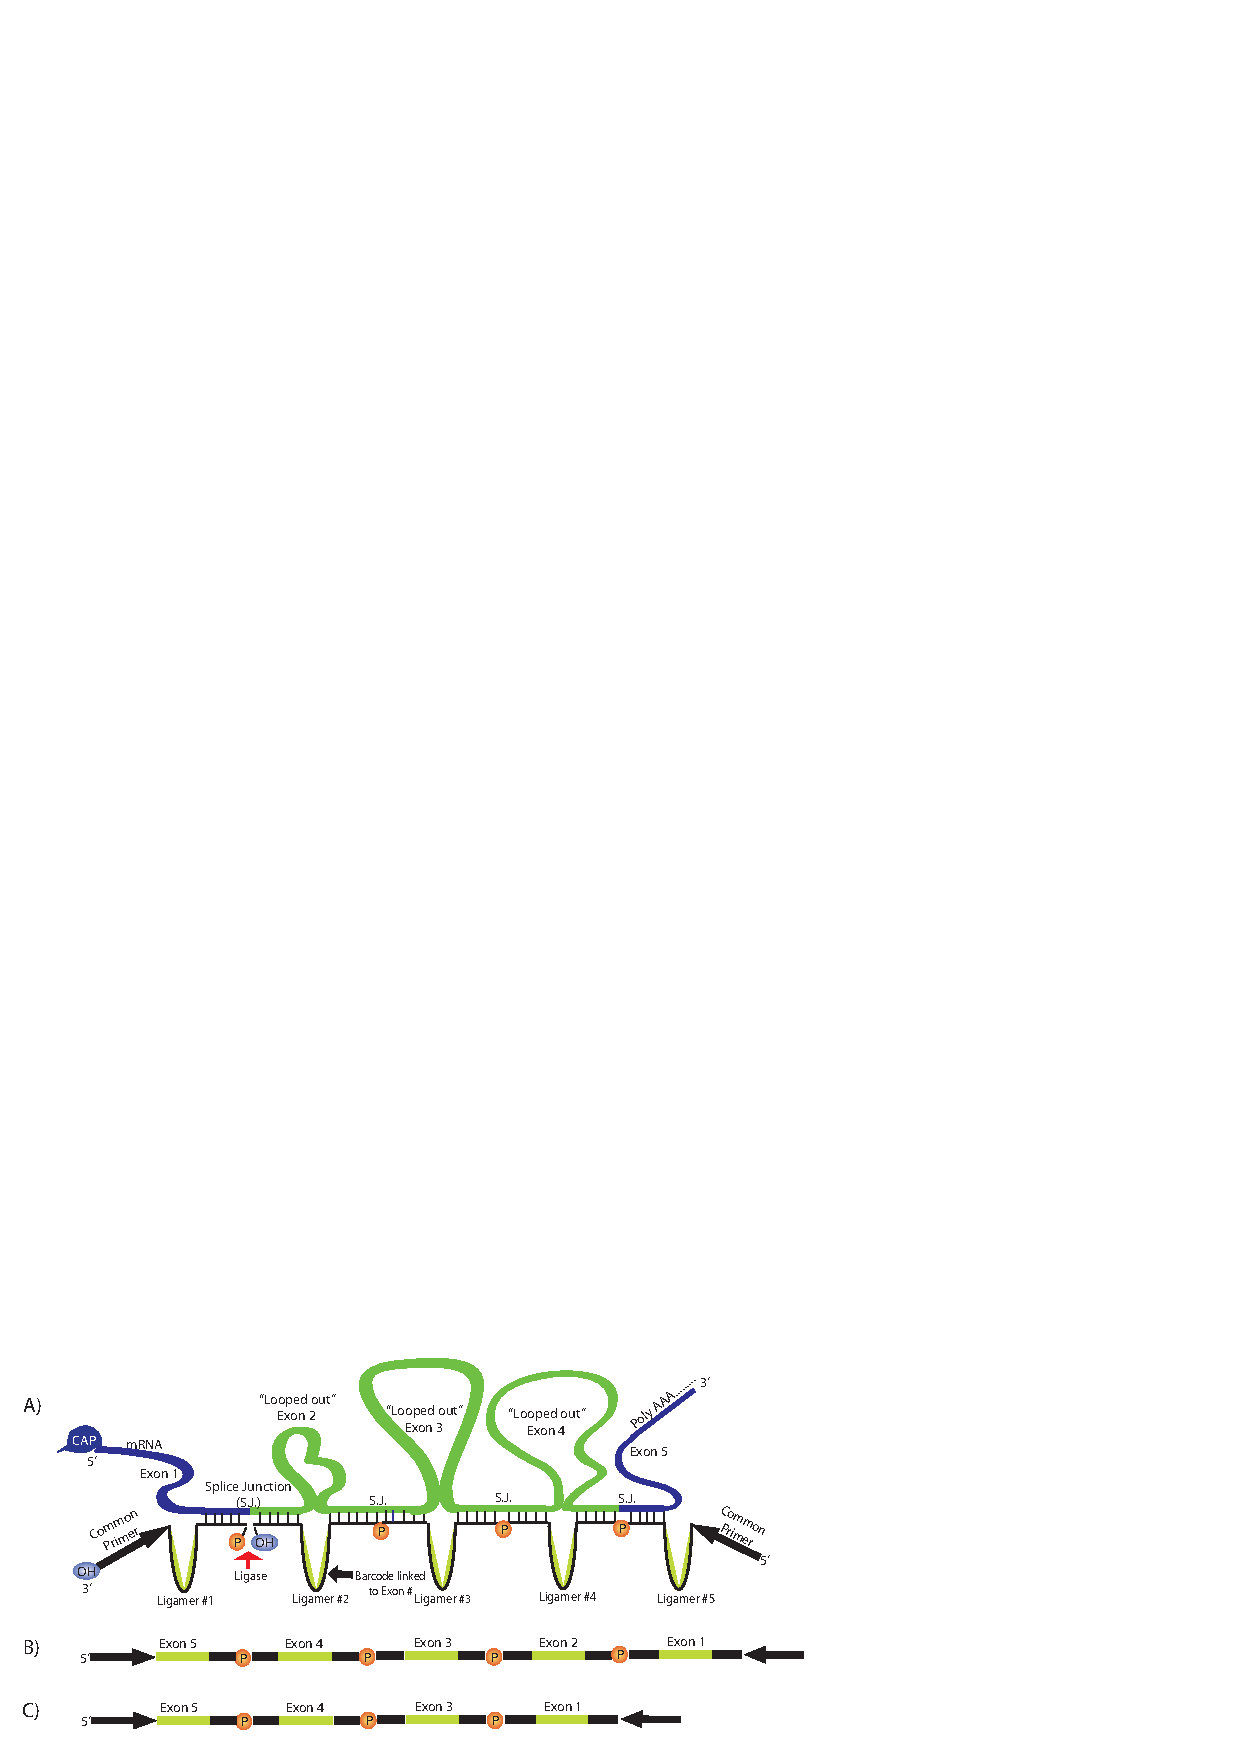
\includegraphics{Figures/Chapter2/OriginalSeqZipDiagram.pdf}
	\caption[Original SeqZip Diagram]
	{
		Original SeqZip Diagram\\
		This is the original concept diagram of the SeqZip methodology. (A) Specific DNA oligos target an mRNA and loop out the RNA sequence. Ligases is added to join the DNA oligos together; (B) \& (C) Two different possibilities of ligation products templated from the RNA in (A), where Exon 2 is an cassette exon.
	}
	\label{fig:Original SeqZip Diagram}
\end{figure}
%% ############# FIGURE

%----------------------------------------------------------------------------------------
\section{Multiplex Gene Study}
%----------------------------------------------------------------------------------------

One of the major goals of developing the SeqZip methodology was investigating potential coordination genome-wide. By genome-wide, what we really mean is to analyze many (or all) of the RNA transcripts in a tissue for evidence of coordinated splicing decisions. When development of the method reached the point that it could be applied in a multiplex study, I did not posses the bioinformatic skills necessary to 1) design ligamers in an automated and high-throughput fashion and 2) identify target transcripts, exons, and sequences to investigate for potential connectivity. Both of these points are discussed later, see <automated ligamer design | appendix> and <ideas on transcript identification for SeqZip coordination investigation | Discussion/Perspective>.

A hypothesis we wanted to use SeqZip to test was that coordination among distant regions of AS in the same transcript is a general phenomenon. It is important to note that we are not limiting our scope of coordination to that between two internal sites of AS (–e.g., cassette or mutually exclusive exon events). From microarrays studies, it has been estimated that approximately 30\% of all AS events involve alternative first and last exons (Bingham et al., 2008).  It is known that, through alternative use of first and last exons, cells can fine-tune a transcript’s untranslated region (UTR) and control many aspects of mRNA regulation including nuclear export, localization, expression, and stability (Hughes, 2006).  In support of the importance of alternative UTRs in tuning of gene expression, a landmark RNA-Seq study demonstrated a high occurrence of alternative first and last exon splicing, with alternative tandem 3’ UTR usage being the most highly tissue-dependent form of AS observed (Wang et al., 2008).  The current model of spatial proximity between 5’ and 3’ UTRs is suggestive of their possible interdependence. In our large-scale analysis, we included genes potentially displaying interdependence between first and last exons. Discovery of interdependence would lead to many questions into how specific combinations of UTRs can influence mRNA processing downstream of AS.


%% ############# FIGURE
\begin{figure}[htbp]
	\centering 
	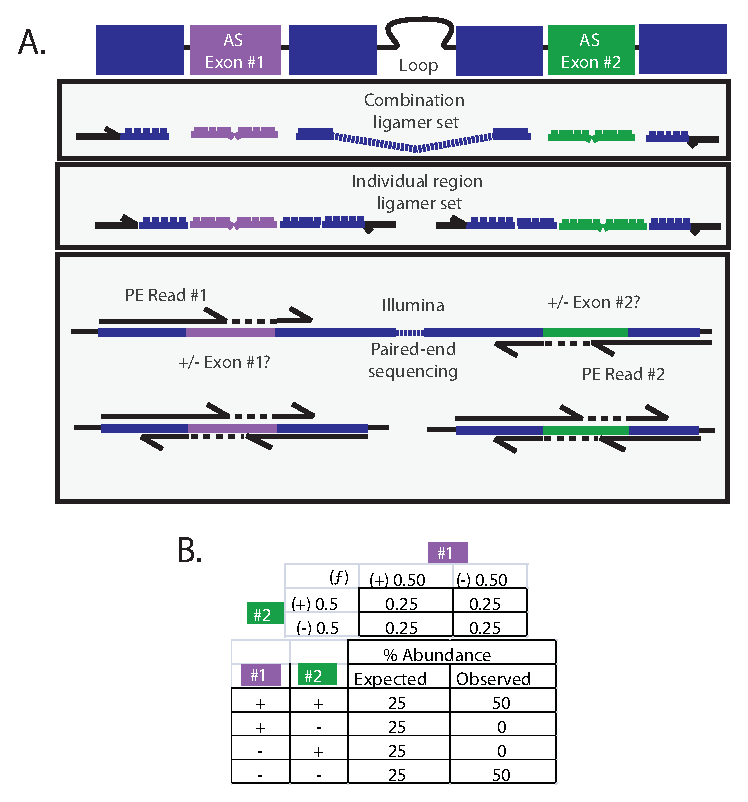
\includegraphics{Figures/Chapter2/10GeneSetSchematic.eps}
	\caption[10 Gene Set schematic]
	{
		10 Gene set schematic\\
		\hl{caption next}
	}
	\label{fig:Original SeqZip Diagram}
\end{figure}
%% ############# FIGURE

In an effort not to let my lack of bioinformatic ability hold back application of SeqZip to many transcripts at once, I designed a series of experiments that I termed a 'multiplex' application of SeqZip. It was based off of a very important paper from the Blencowe lab, where they used AS-sensitive microarrays to investigate transcripts in the Mouse CNS (Fagnani et al. 2007). This paper identified genes displaying tissue-specific splicing patterns, focusing on those with CNS-specific patterns. Once section of their paper focused on "Coordination between AS events belonging to the same genes," and seemed to be the exact type of experiment we were interested in applying the SeqZip method too. Five hundred of the 3,044 genes investigated by their microarrays contained 2–5 alternative exons. Fagnani et all contained an additional data file a list of all pair-wise combinations of alternative exons in the same gene (with that gene having significant expression in >20 different tissues), along with the standard and partial spearman correlations. Using this dataset, I filtered the exon pairs to those with a distance > 350 nt in the final pre-mRNA. I also visualized their transcript achetecture, and EST evidence using NCBIs AceView tool (Thierry-Mieg and Thierry-Mieg 2006). For example, the exons with strong correlation of expression in the Chl1 gene are in the beginning (second exon) and end (fourth from last exon, accession BC060216) with plenty of supporting evidence for these exons being expressed, and skipped.  After combing through the Fagnani data for a group of about 10 genes displaying these characteristics, I designed ligamers for the alternative, and flank constitutive exons. These oligos were then ordered from IDT in a 96-well plate format, pooled according to gene, and used to develop a multiplex approach to applying SeqZip, as well as investigate coordination between these exons, in these genes, using mouse total RNA from brains.

After synthesis, ligamers targeting a particular gene will be pooled at the predetermined appropriate concentration. Poly(A) samples from a treatment condition, cell-, or tissue-type of interest will be isolated.  These samples will be parsed out into individual wells of a 96-well plate, and different ligamer sets will be added to individual wells followed by analysis using SeqZip. Analysis of the resulting FLLPs can be carried out manually using semi-quantitative PCR, followed by denaturing PAGE or by one 454 sequencing run.  After analysis, the lengths of observed FLLPs will be related back to those predicted during ligamer construction.  Our primary data will represent the relative abundance of observed gene-specific isoforms for the cell- or tissue-type examined.

%-----------------------------------
\subsection{Subsection 1}
%-----------------------------------

\begin{table}[h]
\begin{tabular}{|l|r|r|r|r|}
\hline
\textbf{Gene name} & \textbf{nt of mRNA between exons} & \textbf{possible isoforms} & \textbf{Exon 1} & \textbf{Exon 2} \\ \hline
Chl1               & 4665                              & 18                         & 2               & 24              \\ \hline
Mdm1               & 1846                              & 4                          & EDA             & IIICS           \\ \hline
PTPRF-Y            & 1633                              & 4                          & 2               & 13              \\ \hline
Cacna1c            & 1403                              & 4                          & 15              & 21/22           \\ \hline
PTPRF-X            & 936                               & 4                          & 9/10            & 21              \\ \hline
FN1                & 813                               & 8                          & 13/14           & 21/22           \\ \hline
Apbb1              & 802                               & 260                        & 1/2b            & 2/3e            \\ \hline
Agrn               & 736                               & 8                          & 33/34c          & 33/34a          \\ \hline
Exoc7              & 513                               & 4                          & 7               & 13              \\ \hline
Prom1              & 512                               & 4                          & 7               & 9               \\ \hline
Lphn2              & 396                               & 32                         & 19              & 24/25a          \\ \hline
\end{tabular}
  \caption[Genes with big spans in between]{\hl{caption}}
  \label{BigSpanGenes}
\end{table}

%----------------------------------------------------------------------------------------
\section{Determining RNA integrity using SeqZip}\label{sec: SeqZip Intergrity}
%----------------------------------------------------------------------------------------

%-----------------------------------
\subsection{Demonstration of Concept}
%-----------------------------------

%% ############# FIGURE
\begin{figure}[htbp]
	\centering 
	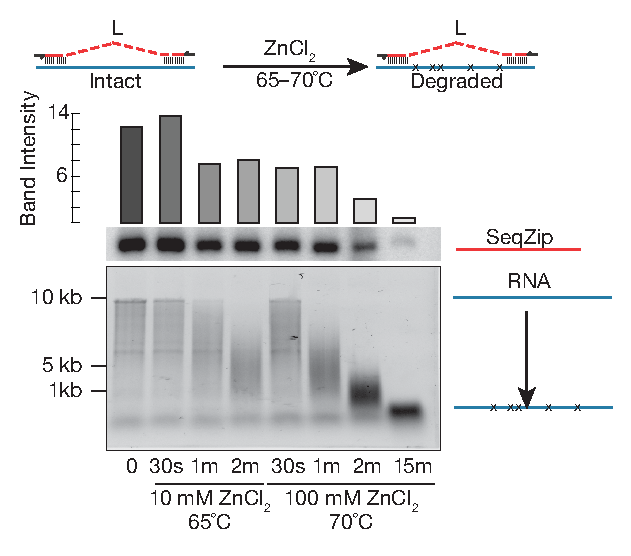
\includegraphics{Figures/Chapter2/DegreadedRNABySeqZip.eps}
	\caption[Ligation product tied to RNA integrity]
	{
		Ligation product tied to RNA integrity\\
		\hl{figure Caption}
	}
	\label{fig:Ligation product and RNA integrity}
\end{figure}
%% ############# FIGURE

\lipsum[1-3]

%% ############# FIGURE
\begin{figure}[htbp]
	\centering 
	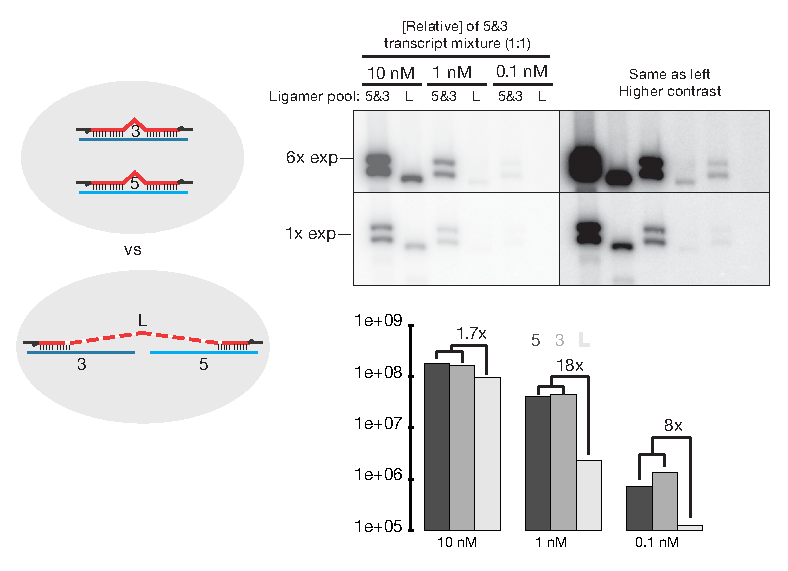
\includegraphics{Figures/Chapter2/TransRNAWithSeqZip.eps}
	\caption[Trans Transcript investigation]
	{
		Trans Transcript investigation\\
		\hl{figure Caption}
	}
	\label{fig:Ligation product and RNA integrity}
\end{figure}
%% ############# FIGURE

%-----------------------------------
\subsection{Investigating HIV viral genome integrity using SeqZip}
%-----------------------------------


%! Base the discussion off the introduction in the HIV paper (Serquiña et al. 2013)

MOV10L1 is implicated in HIV genome stability and intactness. We sought to measure the effects of a point mutant in the ATPase domain of MOV10L1 on the ‘intactness’ of the HIV genome. Viral particles contain two copies of the ssRNA HIV genome. Proteomics studies have measured MOV10L1 and Upf1 in viral particles, implicated these proteins, which are known helicases, in the maintained and infectivity of HIV.

%-----------------------------------
\subsection{Design of HIV ligamers}
%-----------------------------------

Research into the integrity of the HIV RNA genome using SeqZip began with designing a set of ligamers against two different clones. The first clone, targeting transcripts from the M19921 plasmid (so called 'M' clone), and transcripts from the K03455 clone contain nearly identical sequences with respect to the genome itself, and differ mostly in plasmid originating sequences. We targeted a difference in sequence for one site of ligation (Fig3-11A). Three different pools of ligamers were created initially: a Five(5) ligamer pool, with three ligamers design to test for the presence of sequence in the first 1,140 nt of the HIV genome, importantly the first site of ligation in the 5 region pool should contain a mismatch in the K clone sequence; a three(3) pool, testing the last 1,210 nt of the genome, and a Long (L) ligamer pool, also containing three ligamers, but the middle ligamer of which would span the 5 and 3 regions, looping out 8,633 nt of sequence in the middle of the HIV genome. In vitro transcripts were created using both the K and M clone plasmids. These transcripts were added to a background of total MEF RNA, and the SeqZIp assay was performed. Ligation products were successfully amplified from all ligamer pools when using the M clone transcript and all three ligamer pools. Also the abundance of these ligation products, as measured by endpoint PCR, seemed to be spike-concentration dependent. Notably, Ligation products were not obtained from the K clone using either the 5 or L ligamer pools, likely due to the mismatch between the transcript and the ligamers at the site of ligation. Also of note was the appearance of ligation products from purified endogenous virons of the M clone from all three ligamer pools, and the absence of products from virions purified from plasmids containing a defective protein, Gag, essential for viral packaging. 

%% ############# FIGURE
\begin{figure}[htbp]
	\centering 
	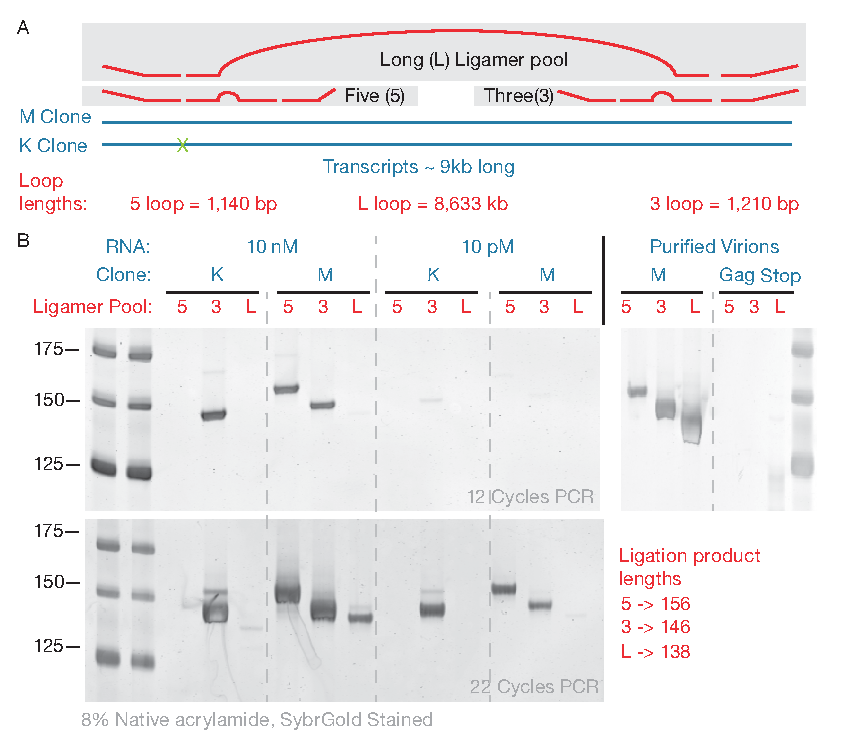
\includegraphics{Figures/Chapter2/HIVviaSeqZip.eps}
	\caption[SeqZip can examine HIV transcript integrity]
	{
		SeqZip can examine HIV transcript integrity\\
		\hl{figure Caption}
	}
	\label{fig:Hiv tx via SeqZip}
\end{figure}
%% ############# FIGURE

%----------------------------------------------------------------------------------------
\section{Continuity of piRNA precursor transcripts}\label{sec: piRNA Precursor SeqZip analysis}
%----------------------------------------------------------------------------------------

%% ############# FIGURE
\begin{figure}[htbp]
	\centering 
	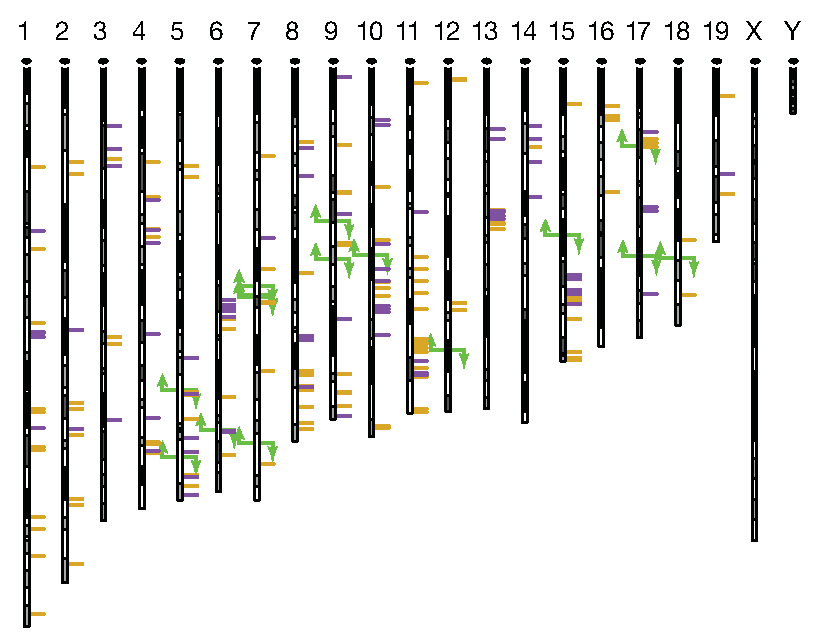
\includegraphics{Figures/Chapter2/PrecursorLocations.eps}
	\caption[piRNA precursor locations]
	{
		piRNA precursor locations\\
		\hl{figure Caption}
	}
	\label{fig:Hiv tx via SeqZip}
\end{figure}
%% ############# FIGURE


%Table 3 1, Just 9 clusters from 5 promoters generate >50% of 14.5 dpp (pachytene) piRNAs
\begin{table}[h]\small
\begin{tabular}{llrrr}
\hline
\textbf{Cluster Name} & \textbf{\begin{tabular}[c]{@{}c@{}}Matched \\ Cluster\end{tabular}} & \textbf{\begin{tabular}[c]{@{}c@{}}Unique-mapping \\ piRNAs @ \\ wt.14dpp\end{tabular}} & \textbf{\begin{tabular}[c]{@{}c@{}}Fraction of \\ pachytene \\ piRNAs\end{tabular}} & \textbf{\begin{tabular}[c]{@{}c@{}}Cumulative\\  pachytene\\  piRNAs\end{tabular}} \\ \hline
17-qA3.3-26735.1      & 17-qA3.3-27363                                                      & 3,021,022                                                                               & 17.2                                                                                & 17.2                                                                               \\
17-qA3.3-27363.1      & 17-qA3.3-26735                                                      & 1,742,695                                                                               & 9.9                                                                                 & 27.2                                                                               \\
9-qC-31469.1          & 9-qC-10667                                                          & 1,006,333                                                                               & 5.7                                                                                 & 32.9                                                                               \\
9-qC-10667.1          & 9-qC-31469                                                          & 272,385                                                                                 & 1.6                                                                                 & 34.5                                                                               \\
7-qD2-24830.1         & 7-qD2-11976                                                         & 652,564                                                                                 & 3.7                                                                                 & 38.2                                                                               \\
7-qD2-11976.1         & 7-qD2-24830                                                         & 280,312                                                                                 & 1.6                                                                                 & 39.8                                                                               \\
6-qF3-28913.1         & 6-qF3-8009                                                          & 564,930                                                                                 & 3.2                                                                                 & 43.0                                                                               \\
6-qF3-8009.1          & 6-qF3-28913                                                         & 180,210                                                                                 & 1.0                                                                                 & 44.0                                                                               \\
2-qE1-35981.1         & NA                                                                  & 1121042                                                                                 & 6.4                                                                                 & 50.4                                                                               \\ \hline
\end{tabular}
  \caption[Just 9 piRNA genes create >50\% of mammalian piRNAs]{\hl{caption}}
  \label{tab:FlyGenesWithManyTx}
\end{table}

%% ############# FIGURE
\begin{figure}[htbp]
	\centering 
	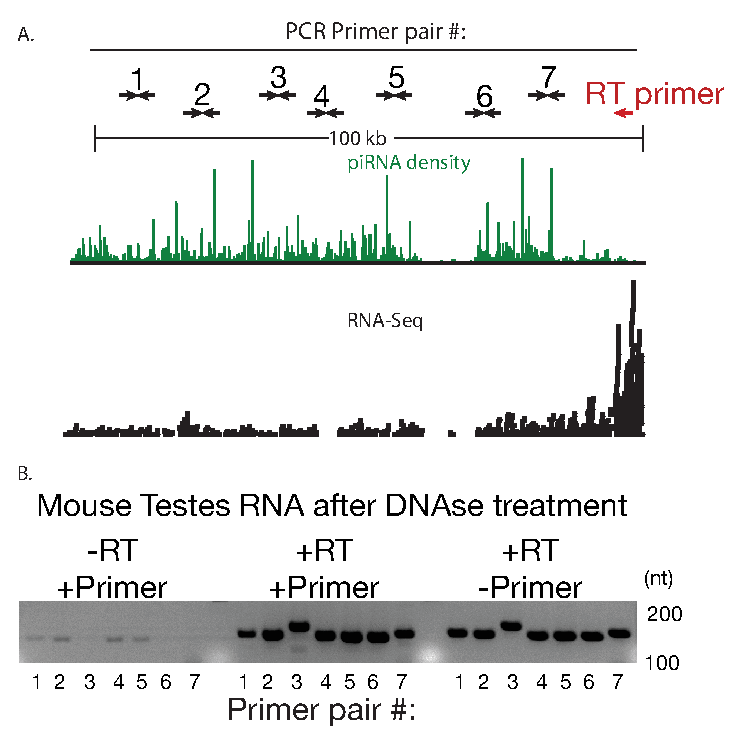
\includegraphics{Figures/Chapter2/RTDoesntWork.eps}
	\caption[pRT Doesn't Work for piRNA precursors]
	{
		RT Doesn't Work for piRNA precursors\\
		\hl{figure Caption}
	}
	\label{fig:Hiv tx via SeqZip}
\end{figure}
%% ############# FIGURE


%% ############# FIGURE
\begin{figure}[htbp]
	\centering 
	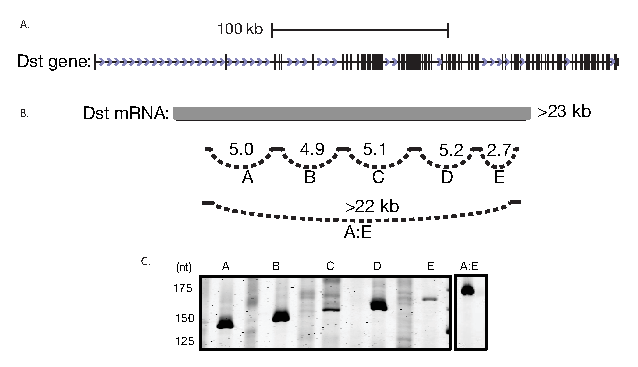
\includegraphics{Figures/Chapter2/dst1.eps}
	\caption[Dst1 by SeqZip]
	{
		Dst1 by SeqZip\\
		\hl{figure Caption}
	}
	\label{fig:Hiv tx via SeqZip}
\end{figure}
%% ############# FIGURE


%% ############# FIGURE
\begin{figure}[htbp]
	\centering 
	\includegraphics{Figures/Chapter2/testesSpecificRnaseqPrecursors.eps}
	\caption[Testes Specific RNA precursor expression]
	{
		Testes Specific RNA precursor expression\\
		\hl{figure Caption}
	}
	\label{fig:Hiv tx via SeqZip}
\end{figure}
%% ############# FIGURE


%% ############# FIGURE
\begin{figure}[htbp]
	\centering 
	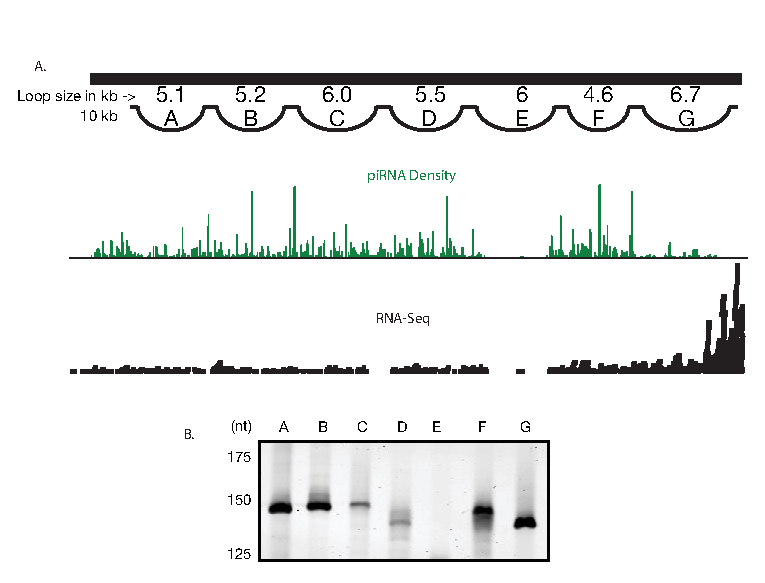
\includegraphics{Figures/Chapter2/piRNAPrecurserAnalyisBySeqZip.eps}
	\caption[piRNA precursor analysis via SeqZip]
	{
		piRNA precursor analysis via SeqZip\\
		\hl{figure Caption}
	}
	\label{fig:Hiv tx via SeqZip}
\end{figure}
%% ############# FIGURE


 
\chapter{SeqZip Publication} 
\label{Chapter3} 
\lhead{Chapter 3. \emph{SeqZip Publication}} 
%----------------------------------------------------------------------------------------
\section{Abstract}\label{c1sec: Abstract}
%----------------------------------------------------------------------------------------

%----------------------------------------------------------------------------------------
\section{Introduction}\label{c1sec: Introduction}
%----------------------------------------------------------------------------------------

%% ############# FIGURE
\begin{figure}[htbp]
	\centering 
	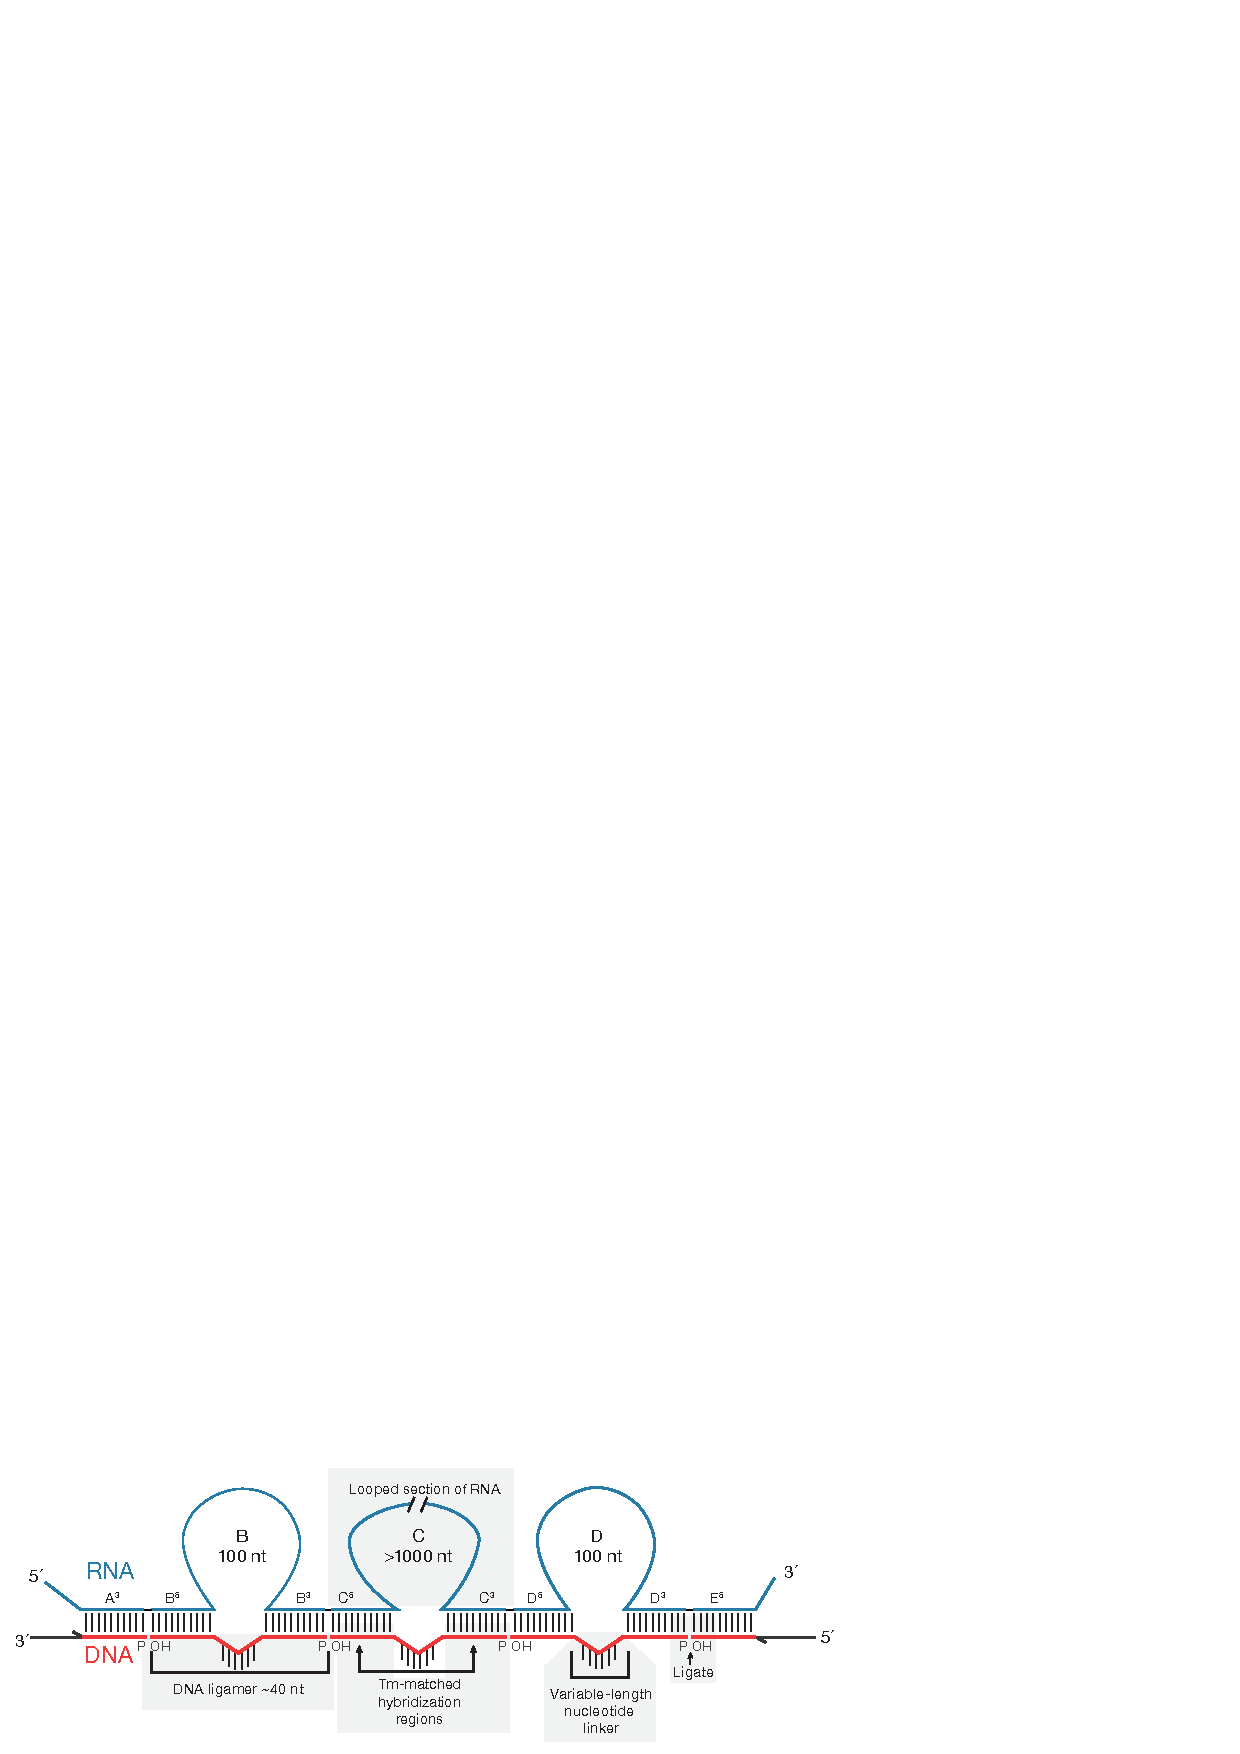
\includegraphics{Figures/Chapter3/Roy2014Fig1.pdf}
	\caption[SeqZip Diagram]
	{
		SeqZip Diagram]\\
		\hl{Insert Figure Text}
	}
	\label{fig:Roy2014 SeqZip Diagram}
\end{figure}
%% ############# FIGURE


%----------------------------------------------------------------------------------------
\section{Results}\label{c1sec: Results}
%----------------------------------------------------------------------------------------

%-----------------------------------
\subsection{Subsection 2}
%-----------------------------------

%% ############# FIGURE
\begin{figure}[htbp]
	\centering 
	\includegraphics{Figures/Chapter3/Roy2014Fig2.eps}
	\caption[SeqZip Diagram]
	{
		Rnl2 Panel]\\
		\hl{Insert Figure Text}
	}
	\label{fig:Roy2014 Rnl2}
\end{figure}
%% ############# FIGURE


%-----------------------------------
\subsection{Subsection 2}
%-----------------------------------

%% ############# FIGURE
\begin{figure}[htbp]
	\centering 
	\includegraphics{Figures/Chapter3/Roy2014Fig3.eps}
	\caption[SeqZip Diagram]
	{
		Rnl2 Panel]\\
		\hl{Insert Figure Text}
	}
	\label{fig:Roy2014 Rnl2}
\end{figure}
%% ############# FIGURE

%----------------------------------------------------------------------------------------
\section{Discussion}\label{c1sec: Discussion}
%----------------------------------------------------------------------------------------
%----------------------------------------------------------------------------------------
\section{Methods}\label{c1sec: Methods}
%----------------------------------------------------------------------------------------

%----------------------------------------------------------------------------------------
\section{Supplemental Text}\label{c1sec: Supplemental Text}
%----------------------------------------------------------------------------------------


\input{Chapters/Chapter4-MolCel2013} 
\chapter{Discussion} % Main chapter title

\label{Chapter 5} % for referencing this chapter elsewhere, use \ref{Chapter X}

\lhead{Chapter 5. \emph{Discussion}} % this is for the header on each page 

%----------------------------------------------------------------------------------------
%	SECTION 1
\section{Future of Dyanmic long RNAs}
%----------------------------------------------------------------------------------------

%•	Talk about my path during PhD
%•	Mention BG’s paper New Insights from Existing Sequence Data: Generating Breakthroughs without a Pipette AM Plocik, BR Graveley Molecular cell 49 (4), 605-617
%•	Discuss importance of BigData and being able to analyze in parallel, looking for genome wide changes
%High resolution transcriptome analysis
%•	Implications for discrination past one's DNA as it is the actual PRODUCT of the DNA and the actual biology (or at least closer to the functional biology) that is going on inside of every person
%25Full length analysis of RNAs
%Long Range RNA interactions
%•	Discuss long range RNA secondary structure and implecations of regulating alternative splicing (See Li, S., & Breaker, R. R. (2013). Eukaryotic TPP riboswitch regulation of alternative splicing involving long-distance base pairing. Nucleic acids research, 41(5), 3022–31. doi:10.1093/nar/gkt057) and Reg of AS by long RANGE SS folder in Mendeley
%Signal and noise separation


Deep sequencing of transcriptomes has revolutionized biology. Previously, transcript discovery was a cumbersome task. Transcript identification and characterization involved significant labor, cost, and materials. In the mid-90's, microarray technology \citep{Schena1995a} gave us a tantalizing glimpse into how genes were expressed, but were limited to probed, and therefore known, sequences. However, the green and red landscapes of a microarray analysis hinted at incredible complexity\textemdash a complexity that would have to wait for technology to catch up.

Like many transformative technologies, RNA-seq was made possible by incremental improvements to numerous supportive technologies such as: 1) digital optics, 2) microscopy, 3) slide chemistry and on-slide PCR and 4) nucleic-acid alignment. A HiSeq 2500 relies on all of these technologies (and others) to produce the 100M+ sequences that allow Scientists to peer every day into the transcriptional output of a genome.

In the past 5 years, biologists have started to think way beyond mRNAs and small RNAs. The former captured out interest for 30+ years \citep{Furuichi1975,Wei1975}, and the later has been on a run-away trail since capturing out attention in 1998 \citep{Fire1998}. HTS has added long RNAs (among others) to these classes of gene RNA products. 

Being such a novel area of extremely basic research, and to borrow a few seemingly inane but rather insightful trio of phrases from the United States Secretary of Defense Donald Rumsfeld \citep{Rumsfeld2011}, their remain at least three important areas of knowledge concerning long RNAs of the transcriptome: 
\hyperref[subsec: The Known Knowns]{''The Known Knowns''}; 
\hyperref[subsec: The Known Unknowns]{''The Known Unknowns''}; 
and the \hyperref[subsec: The Unknown Unknowns]{''The Unknown Unknowns''}.

%-----------------------------------
%	SUBSECTION 1
\subsection{The Known Knowns}\label{subsec: The Known Knowns}
%-----------------------------------

At this point, it is important to remember that in this document \textit{long RNAs} may also refer to products containing characteristics of traditional mRNAs, that is a 5\textprime~m7G Cap, ligated exons, and a Poly(A) tail. However, many of these long mRNAs are extemely dynamic. So much so that until HTS and RNA-Seq, comprehensive investigation of their complexity was not possible.


\begin{description}
	\item[Pervasive transcription]
	Here you can put some information from ENCODE and your thoughts on it.

	\item[Tissue and cell specificity]
	Your feelings on Specificity of long RNA expression

	\item[Functional]
	We \textit{know} that some long RNAs are functional. What are these?

	\item[Chromatin regulation]
	We also know that some long RNAs regulation Chromatin structure. What are your feelings as to the importance of this fact?

	\item[PTGS]
	Long RNAs ability to do post transcriptional gene regulation, including piRNAs, and Xist, etc....

\end{description}

%-----------------------------------
%	SUBSECTION 2
\subsection{The Known Unknowns}\label{subsec: The Known Unknowns}
%-----------------------------------


\begin{description}
	\item[How are they important?] 
	Conservation of these things is not obvious - if they are not conserved - are they important? Maybe talk about how MALAT1 is highly expressed, but seems to be dispensable.

	\item[What regulates their tissue-specific expression?]
	Do they important some of the special sauce that makes tissues different from one other, more so then the mRNAs changes which can be extreme, but not terribly so....

	\item[]  

\end{description}

%-----------------------------------
%	SUBSECTION 2
\subsection{The Unknown Unknowns}\label{subsec: The Unknown Unknowns}

This is the area of knowledge keeps many motivated to perform basic research every day. What secrets does the transcriptome have in store that we haven't even \textit{thought} about? Only through pushing the boundaries of the last two sections can we begin to think beyond the edge of map and formulate testable hypothesis. Here I propose a few outlandish ideas for Unknown Unkowns.



%----------------------------------------------------------------------------------------
%	SECTION 1
\section{Ligation-based investigation of long RNAs}
%----------------------------------------------------------------------------------------
%-----------------------------------
%	SUBSECTION 1
\subsection{SeqZip Other Applications}
%-----------------------------------
%-----------------------------------
%	SUBSECTION 2
\subsection{SeqZip Technical Improvements}
%-----------------------------------

\begin{itemize}
	\item Use of T39A mutation to aliviate penultimate 2´ OH requirement of T4 Rnl2 (See Nandakumar...Lima, Cell 2006)
	\item Use of thermostable ligase, allowing for multiple rounds of ligation. Need a good reference, DO NOT USE Ref 27 from Conze et al 2009!
	\item Elevated ligation temperatures, minimizing blut-ended NTL events
	\tem Make a note into the future directions that you would like to explore LNA’s at the 3´OH pisition of all ligation results, leading to increased ligation efficiency, however both this and the use of penultimate 2´ OH (Ribosome) suger in your ligamers would lead to added costs, and the latter maybe better served with a T39A mutation. Giggity }
	\item Digital PCR of the PCR products ala \citep{Shiroguchi2012a}. 
\end{itemize}

%-----------------------------------
%	SUBSECTION 3
\subsection{SeqZip Alternatives}
%-----------------------------------
%----------------------------------------------------------------------------------------
%	SUBSECTION 1
\section{Mammalian piRNA-precursors, a special type of long RNA}
%----------------------------------------------------------------------------------------


%Unanswered questions/issues of the resources paper?

%-----------------------------------
%	SUBSECTION 1
\subsection{What are they doing?}
%-----------------------------------

%Interaction w/ ribosomes?

%-----------------------------------
%	SUBSECTION 2
\subsection{How are they generated?}
%-----------------------------------

%Interaction w/ ribosomes?
%How does cell partition prepachytene transcripts to mRNA or piRNA use?

%-----------------------------------
%	SUBSECTION 3
\subsection{Why should we care?}
%-----------------------------------

% The references are stored in the file named "library.bib.bib"
%\bibliography{library.bib}  


%----------------------------------------------------------------------------------------
%	THESIS CONTENT - APPENDICES
%----------------------------------------------------------------------------------------

\addtocontents{toc}{\vspace{2em}} % Add a gap in the Contents, for aesthetics

\appendix % Cue to tell LaTeX that the following 'chapters' are Appendices
\label{hd:Appendicies}
% Include the appendices of the thesis as separate files from the Appendices folder
% Uncomment the lines as you write the Appendices

% Appendix A

\chapter{Appendix - Misc Information} % Main appendix title

\label{AppendixA} % For referencing this appendix elsewhere, use \ref{AppendixA}

\lhead{Appendix A. \emph{Appendix Title Here}} % This is for the header on each page - perhaps a shortened title

%----------------------------------------------------------------------------------------
\section{Equations}\label{sec:Equations}
%----------------------------------------------------------------------------------------

\subsection{Determining [RNA] from $^{32}$P-$\alpha$-UTP used during vitro transcription}

{\tiny{
\begin{eqnarray*}
\mu \mbox{M} = \left( \frac{\mbox{pmol}}{\mu\mbox{L}}\right)
      = \left( \frac{\mbox{cpm after purification} \times \mbox{dilution factor}}{\mbox{cpm before purification} \times \mbox{dilution factor}} \right)
      \times \left( \frac{\mbox{mol UTP in original reaction}}{\mbox{Reaction Volume }} \right) \times \left( \frac{1}{\mbox{Number UTPs in transcript}} \right) \times 10^{-12} 
\end{eqnarray*}
}
}
%Or you can write the above equation as 

%\begin{eqnarray*}
%\mu \mbox{M}  =  \left( \frac{\mbox{pmol}}{\mu\mbox{L}}\right)
     %& = & \left( \frac{\mbox{cpm after purification} \times \mbox{dilution factor}}{\mbox{cpm before purification} \times \mbox{dilution factor}} \right)\\
%      && \times \left( \frac{\mbox{mol UTP in original reaction}}{\mbox{Reaction Volume}} \right)\\
 %     && \times \left( \frac{1}{\mbox{Number UTPs in transcript}} \right) \times 10^{-12} 
%\end{eqnarray*}
%%%%%%%%%%%%%%%%%%%%%%%%%%%%%%%%%%%%%%%%%%%%%%%%

\ \\
\ \\

\subsection{Determining [RNA] based on A$_{260}$}


$$
\mbox{[RNA in M]} = \left( \frac{\mbox{A}_{260} \times \mbox{Dilution Factor}}
                           {10,313 < \mbox{note 1}> \times \mbox{ nucleotides in message}} \right) 
$$
note 1: This value represents an average RNA extinction ($\epsilon$) coefficient value \\

\subsection{Normalize oxidized small RNA libraries size to time-matched unoxidized library}

NB: this equation assumes calibration against a specific time-point ,
in this case data obtained from '6wk' tests.

\begin{eqnarray*}
     \mbox{unox }\tau \mbox{ norm}_1 & = & \left(         
                        \frac{\left( \frac{\displaystyle\sum \mbox{miRNA reads } \tau}{\displaystyle \sum \mbox{miRNA reads 6wk} } \right) \times \mbox{ depth 6wk} }{1,000,000}              
                                          \right)\\
\mbox{ox }\tau \mbox{ norm}_1 & = &   \mbox{unox }\tau \mbox{ norm}_1 \times
                                 \left(
                                  \frac{\displaystyle \sum \mbox{oxidized shared } \ge \mbox{23 nt reads}}{\displaystyle \sum \mbox{unoxidized shared } \ge \mbox{23 nt reads}}
                                 \right)                                         
\end{eqnarray*}


%\chapter{Appendix B: Automated Ligamer Assembly}\label{Appendix:AutoMatedLigamerAssembly} 
\lhead{Appendix B. \emph{Perl Script for Automated Ligamer Assembly}} 

\section{Installation}

Major Steps:
\begin{itemize}
	\item  Create an input csv file with required information
	\item  Run this information sequentially through the scripts
	\item  Use the results to order oligos from IDT
\end{itemize}

Required Tools:
\begin{itemize}
	\item  Perl
	\item  BioPerl
	\item  Ensembl Perl APIs
	\item  String::Random Perl Package
\end{itemize}

Items to future improvements
\begin{itemize}
	\item Use Ensembl Database to initilize queries
	\item Make the use of BioPerl more flexible
	\item Make more web-friedly
\end{itemize}

Helpful hints on installing BioPerl and Emsembl Perl APIs:

\lstset{language=BASH}
\begin{lstlisting}
	## Install BioPerl, use git
	    cpan App::cpanminus # First prep cpan
	    cpanm DBI ## Install necessary DBI perl module
	    mkdir ~/src; cd ~/src
	    git clone git://github.com/bioperl/bioperl-live.git
	    cp ~/.bash_profile ~/.bash_profile.bak
	    echo -e 'PERL5LIB=$HOME/src/bioperl-live:$PERL5LIB' >> ~/.bash_profile
	    source ~/.bash_profile
	# Install ensembl perl apis
	    mkdir ~/src; cd ~/src
	    wget ftp://ftp.ensembl.org/pub/ensembl-api.tar.gz
	    tar xvfz ensembl-api.tar.gz
	# Add locations to perlfile libs to $PATH
	    echo -e '
	    PERL5LIB=${PERL5LIB}:${HOME}/src/ensembl/modules
	    PERL5LIB=${PERL5LIB}:${HOME}/src/ensembl-compara/modules
	    PERL5LIB=${PERL5LIB}:${HOME}/src/ensembl-variation/modules
	    PERL5LIB=${PERL5LIB}:${HOME}/src/ensembl-functgenomics/modules
	    export PERL5LIB' >> ~/.bash_profile
\end{lstlisting}
%----------------------------------------------------------------------------------------
\section{Example Input Format}
%----------------------------------------------------------------------------------------
\begin{landscape}
Here is an example input file to create ligamers investigating the \textit{Gria3} gene in Rats:

\begin{table}[!h] % Ligamer Input Example Top
   \label{Appendix:tab:Example Input Top}
   \footnotesize
  \begin{tabular}{lcccccccc}
  \# Comment lines are ignored\\
  \#Gene name\\
  ~GRIA3\\
  \# PCR primers used - Solexa PE adaptor sequences\\
  \# Five prime\\
  PCR-Primer-5'-ATCTGAGCGGGCTGGCAAGGC\\
  \#Three Prime\\
  PCR-Primer-3'-GCCTCCCTCGCGCCATCAGA\\
  \end{tabular}

   \end{table}

\begin{table}[!h] % Ligamer Input Example Bottom
   \label{Appendix:tab:Example Input Bottom}
   \footnotesize
\begin{tabular}{lcccccccc}
ExonId                                                                          & LigID & Name    & Strand & Code & TargetPrime & bedLoc & SetID & ConstID \\
<Gria3\_201/202-Shared-I14                                                        & 10        & rn4 & minus  & TC                   & 5                       & X:127903250-127903350 & NANNNNNN        & 201\_2\_intron    \\
<Gria33\_201/202-Shared-I14                                                        & 9         & rn4 & minus  & T                    & 3                       & X:127903210-127903249 & NNNNNNNN        & 201\_2\_intron    \\
<Gria33\_201/202-E15                                                               & 8         & rn4 & minus  & TC                   & 5                       & X:127914822-127915069 & NNNNNNN         & 201,202           \\
<Gria33\_202-I14:15                                                                & 7         & rn4 & minus  & I                    & N                       & X:127912345-127914821 & TACACAT         & 202               \\
<Gria33\_202-E14                                                                   & 6         & rn4 & minus  & I                    & N                       & X:127912230-127912344 & ACCCCAG         & 202               \\
<Gria33\_201-I14:15                                                                & 5         & rn4 & minus  & I                    & N                       & X:127897499-127914821 & CGCGCAC         & 201               \\
<Gria33\_201-E14                                                                   & 4         & rn4 & minus  & I                    & N                       & X:127897384-127897498 & GTCTCAA         & 201               \\
<Gria33\_202-I13:14                                                                & 3         & rn4 & minus  & I                    & N                       & X:127896828-127912229 & ACCGATT         & 202               \\
<Gria33\_201-I13:14                                                                & 2         & rn4 & minus  & I                    & N                       & X:127896828-127897383 & CGCTATG         & 201               \\
<Gria33\_201/202-E13                                                               & 1         & rn4 & minus  & T                    & 3                       & X:127896580-127896827 & NNNNNNN         & 201,202          
\end{tabular}

   \end{table}

\end{landscape}
%----------------------------------------------------------------------------------------
\section{Ligamer Assembler Source Code}\label{apx: Ligamer Assmembler}
%----------------------------------------------------------------------------------------

\lstinputlisting[language=PERL]{Appendices/ligamerAssembler.pl}


%\chapter{Automated Ligamer Assembly}\label{AppendixC} 
\lhead{Appendix C. \emph{Perl Script for Automated Ligamer Assembly}} 

\section{Installation}

Major Steps:
\begin{itemize}
	\item  Create an input csv file with required information
	\item  Run this information sequentially through the scripts
	\item  Use the results to order oligos from IDT
\end{itemize}

Required Tools:
\begin{itemize}
	\item  Perl
	\item  BioPerl
	\item  Ensembl Perl APIs
	\item  String::Random Perl Package
\end{itemize}

Items to future improvements
\begin{itemize}
	\item Use Ensembl Database to initilize queries
	\item Make the use of BioPerl more flexible
	\item Make more web-friedly
\end{itemize}

Helpful hints on installing BioPerl and Emsembl Perl APIs:

\lstset{language=BASH}
\begin{lstlisting}
	## Install BioPerl, use git
	    cpan App::cpanminus # First prep cpan
	    cpanm DBI ## Install necessary DBI perl module
	    mkdir ~/src; cd ~/src
	    git clone git://github.com/bioperl/bioperl-live.git
	    cp ~/.bash_profile ~/.bash_profile.bak
	    echo -e 'PERL5LIB=$HOME/src/bioperl-live:$PERL5LIB' >> ~/.bash_profile
	    source ~/.bash_profile
	# Install ensembl perl apis
	    mkdir ~/src; cd ~/src
	    wget ftp://ftp.ensembl.org/pub/ensembl-api.tar.gz
	    tar xvfz ensembl-api.tar.gz
	# Add locations to perlfile libs to $PATH
	    echo -e '
	    PERL5LIB=${PERL5LIB}:${HOME}/src/ensembl/modules
	    PERL5LIB=${PERL5LIB}:${HOME}/src/ensembl-compara/modules
	    PERL5LIB=${PERL5LIB}:${HOME}/src/ensembl-variation/modules
	    PERL5LIB=${PERL5LIB}:${HOME}/src/ensembl-functgenomics/modules
	    export PERL5LIB' >> ~/.bash_profile
\end{lstlisting}


%----------------------------------------------------------------------------------------
\section{Example Input Format}
%----------------------------------------------------------------------------------------

%\newgeometry{margin=1cm} % modify this if you need even more space
\begin{landscape}
Here is an example input file to create ligamers investigating the \textit{Gria3} gene in Rats:
\input{Tables/exampleLigamerAssemblerInput.tex}
\end{landscape}
%\restoregeometry


%----------------------------------------------------------------------------------------
\section{Ligamer Assmebly Source Code}\label{apx: Ligamer Assmembler}
%----------------------------------------------------------------------------------------

\lstset{language=PERL}
\begin{lstlisting}
#! /usr/bin/perl

#Pre requisites
# These are working on 02/19/13
use lib "/home/royc/perl5/lib/perl5/"; # BioPerl location
#use lib "/home/royc/lib/ensembl.perl.zpi/ensembl/modules"; #ensembl packages

=head1 Ligamer Assembler

	This script will automatically create ligamers.

=head2 Contact information

	Script made by Christian Roy, Umass Medical School
	christian.roy@umassmed.edu

=cut

use strict; # To help wtih variable control
use warnings; # To help me catch mistakes

use Bio::EnsEMBL::Registry; # To load remote EnsEMBL Registry
use Bio::EnsEMBL::Slice; # To retreave sequences from EnsEMBL registry
use Bio::DB::Fasta; # BioPerl tool to retreave sequnce from local FastA file
use Bio::SeqFeature::Primer; # BioPerl Tool for Tm normalization
use Cwd; # To retreave current working directory information

my $dir = getcwd; # Assign current working directory to scalar
my $timestamp = localtime(); # Grab the time at script start

## Variables
my 	(
	$file_input, # Name of specified input file
	$output_file, # Name of file to print results too
	$species, # The species to grab from Ensembl
	$strand, # The strand to grab for ligamer sequences
	$working_sequence, # The slice sequence variable
	$line_counter, #Keep track of stepping through input file
	@arguments, # Keep track of input arguments
	$fa_reference, # Fill if using a local FASTA Reference file
	$chr, # Obvious
	$coordinates, # Interim variable for splitting UCSC
	$start, # obvious
	$end, # Obvious
	$gene, # target gene name
	$lig_location, # Ligamer prime variable
	$target_prime, # Broad variable to define ligamer type - see man
	$UCSCcoordinates, # Obvious
	$pcrsequence, # fill with appropriate PCR sequence for terminal oligos
	$barcode, # Fill will barcode for sequence between regions of comp.
	$note_line, # Fill with notes for a ligamer query
	$three_prime_PCR_sequence, # Fill with three prime PCR sequence
	$five_prime_PCR_sequence, # Fill with five prime PCR sequence
	$lig_joiner_code, # Internal varialbe for assembling ligamers see man
	$set, # Move set assembly information input to output file
	);

#Variables with Defaults
my $verbose=0; # Verbose loading of ensembl databases
my $db_version=62; # Default database version for ensembl database loading
my $temp="58"; # Defalt temp for Tm normalization
my $salt="0.05"; # Default salt concetration for Tm calculation in M
my $lig_conc="0.00000025"; # Defeult ligamer conc for Tm calc in M
my $man_print=0; # for printing manual information
my $help_print=0; # For printing help informatio to HTML file
my $ligamer_name=0; # Internal variable for sequental numbering of ligamers
my $remote=0; # set to 1 for ensembl database loading
my $control_length=20; # Default length for control variables in nt
my $plname=$0; # assign $plname scalar to script name (for help printing)

#Print Usage information if nothing is entered at commandline
if (@ARGV==0) {system "pod2text $0 | less"; die}

=head2 Usage


	-hp = Print HTML POD data for scriptname
	-mp = Print and view Manual POD data for scriptname
	-i [File] = File Input
	-o [File] = File output
	-v [#] = Verbose for Ensembl loading
	-d [#] = data_base version for Ensembl loading
	-t [#] = Temp in degrees celcius
	-salt [#] = Salt concentration for Tm in mM
	-lig_conc [#] = Ligamer concentration for Tm in nM
	-c [#} = Minimum length for Control ligamers (default=20)

=cut
## Finish message if run with no arguments

#Parse the command line
while(@ARGV>0)
{
  @arguments = @ARGV;  #Store the command line for printing later

  my $next_arg=shift(@ARGV);

  if ($next_arg eq "-hp") { # Do you want to print HTML POD Data?
    $help_print=1;
    }
  if ($next_arg eq "-mp") { # Do you want to print a manual?
    $man_print=1;
    }
  if ($next_arg eq "-i") { # What is the name of the input file?
    $file_input = shift @ARGV;
   }
  if ($next_arg eq "-f") { #n Name of the fasta file your sequences are in?
    $fa_reference = shift @ARGV ;
    }
  if ($next_arg eq "-r") { # Do you want to fetch sequences from ensembl?
    $remote = 1
    }
  if ($next_arg eq "-o") { # Name of output file
    $output_file = shift(@ARGV);
    }
  if ($next_arg eq "-v") { # Do you want to see the ensembl load data?
    $verbose = shift @ARGV;
    }
  if ($next_arg eq "-d") { # What version of ensembl do you want to use?#
    $db_version = shift @ARGV;
    }
  if ($next_arg eq "-t") { # What temperature in degrees C do you want to norm ?
    $temp = shift @ARGV;
    }
  if ($next_arg eq "-salt") { # Salt concentration for Tm calculations?
    $salt = shift @ARGV ;
    $salt = $salt / 1000; # from micro Molar to Molar
    }
  if ($next_arg eq "-lig_conc") { # Concentration for Tm calculations?
    $lig_conc=shift@ARGV;
    $lig_conc = $lig_conc / 1000000000; # nM to M
    }
  if ($next_arg eq "-c") { # What length would you like (min) for control ligs?
    $control_length = shift @ARGV ;
    $control_length = $control_length-1
    }
} ## Finish Parsing the command line

###################### POD HELP SUBROUTINE CALLS################################
my $scriptname=$0;
podhelp( $scriptname, $help_print, $man_print, $dir);
##################### POD HTML Subroutine CALLS#################################

#################### open the ensembl registry#################################
my $db;
if ($fa_reference) {
  $db = Bio::DB::Fasta->new($fa_reference);
  }

if ($remote==1) {
  $db = ensembl_database($verbose, $db_version)
  }
################################################################################
#open the output file
open (OUT, '>'.$output_file) || die "The output file could not be created.\n";
## Print the headers
print OUT
# Start with general assembler information
">Source Program\t",$dir,$0,"\n".
">Date Run \t$timestamp \n".
">Arguments entered \t", "@arguments"," \n".
">Input filename \t$file_input\n".
">Output filename \t$output_file\n".
">Control Seq Length \t$control_length plus 1\n".
">Normalization temperature \t$temp\n".
##### now all on 1 line print the ligmaer-specific information
">Gene\t". #1
"Ligamer_Number\t". #2
"Species\t". #3
"Strand\t". #4
"Ligamer Joiner Code\t". #5
"Target Prime\t". #6
"UCSC coordinates\t". #7
"PCR Used\t". #8
"Barcode Used\t". #9
"Total Query span\t". #10
"Five Prime Sequence\t". #11
"5 Prime Length\t". #12
"Five Prime Tm\t".
"3 Prime Sequence\t".
"3 Prime Length\t".
"3 Prime Tm\t".
#"Ligamer Identifier\t".
"Ligamer Sequence\t".
"Ligamer Length\t".
"Notes\t".
"Set\t".
"\n";
################################################################################
## open the input file
open (INPUT, $file_input) || die "The file $file_input couldn't be opened.\n";
###############################################################################

#################read and analyze each line of the input file #################
while (my $line=<INPUT>) { ## starting brace to read through csv

  if ($line=~/^#/){next} #skips comments
  if ($line=~/^>/){print OUT $line; next} #skips and trans.these lines
  if ($line=~/^~/){$line=~s/~//;chomp $line; $gene=$line;} # find gene identifier
  $gene=~s/[\s]+//g;
  if ($line=~/^\@/){chomp $line;$note_line=$line;next} #store notes

  chomp $line;

  if ($line=~/^PCR-Primer-5'-/g) { #Find the 5 adaptor
    $five_prime_PCR_sequence=$line;
    $five_prime_PCR_sequence=~s/PCR-Primer-5'-//;
    $five_prime_PCR_sequence=~s/[\s]+//g;
    print OUT ">5_pcr\t".$five_prime_PCR_sequence."\n";
    next
    }

  if ($line=~/^PCR-Primer-3'-/) {## find the 3 adaptor
    $three_prime_PCR_sequence=$line;
    $three_prime_PCR_sequence=~s/PCR-Primer-3'-//;
    $three_prime_PCR_sequence=~s/[\s]+//g;
    print OUT ">3_pcr\t".$three_prime_PCR_sequence."\n";
    next
    }

  if ($line=~/^</) {#ligamer query lines start with a '<'
    unless ($note_line) {$note_line=" ";}

    my $lig_joiner_code;
    my $slice_sequence;

    $line_counter++;

     (
     $gene,
     $species,
     $strand,
     $lig_location,
     $target_prime,
     $UCSCcoordinates,
     $barcode,
     $set
     ) = parse_the_line($line);

    $lig_location = uc $lig_location;

    # Parse the ligamer query line
    ($chr, $start, $end)= parse_coordinates($UCSCcoordinates);


    my $target_seq_length = ($end-$start);

############ Get genomic slice from ensembl registry ###############
    if ($remote==1) {
      $slice_sequence =
        get_genomic_sequence
        (
        $chr,
        $start,
        $end,
        $species,
        $db,
        )
      }
#####################################################################

############ Get the genomic slice from local Fasta #################
    if ($fa_reference) {
      #$chr="chr".$chr;
      my $obj = $db -> get_Seq_by_id($chr);
      $slice_sequence = $obj -> subseq ($start => $end);
      }
####################################################################

#### get the correct orientation
    my ($working_sequence) =
      revcom_slice_based_on_strand
        (
         $strand,
         $slice_sequence
         );

  # Get the T5 end
    my ($T5_seq, $T5_tm, $T5_seq_length)=
      obtain_T5_tm_sequence
	  (
	  $working_sequence,
	  $temp,
	  $lig_location,
	  $control_length,
	  $salt,$lig_conc
	  );
  # Get the T3 end
    my ($T3_seq, $T3_tm, $T3_seq_length) =
      obtain_T3_tm_sequence
	  (
	  $working_sequence,
	  $temp,
	  $lig_location,
	  $control_length,
	  $salt,
	  $lig_conc
	  );

  #start to build your working HASH
    my %common =
      (
      working_sequence		=> $working_sequence,
      temp			=> $temp,
      UCSCcoordinates		=> $UCSCcoordinates,
      UCSC_chr			=> $chr,
      UCSC_start		=> $start,
      UCSC_end			=> $end,
      gene 			=> $gene,
      ligamer_name 		=> $ligamer_name,
      species 			=> $species,
      strand			=> $strand,
      target_prime		=> $target_prime,
      five_prime_PCR_sequence	=> $five_prime_PCR_sequence,
      three_prime_PCR_sequence	=> $three_prime_PCR_sequence,
      barcode			=> $barcode,
      target_seq_length		=> $target_seq_length,
      seed			=> $control_length,
      T3_seq			=> $T3_seq,
      T3_tm			=> $T3_tm,
      T3_seq_length		=> $T3_seq_length,
      T5_seq			=> $T5_seq,
      T5_tm			=> $T5_tm,
      T5_seq_length		=> $T5_seq_length,
      notes			=> $note_line,
      set			=>$set,
      );

    if ($lig_location eq "T" && $target_prime eq "5") { #Terminal 5 targeted
      #Advance the ligamer number
      $ligamer_name++;
      $common{ligamer_name} = $ligamer_name;
      # Add to the hash table
      $lig_joiner_code = "T-5";
      $common {lig_joiner_code} = $lig_joiner_code;
      my %lig_results = Terminal_5(%common);
      my %final = ligamer_piece_joiner(%lig_results);
      my %bed_output = %final;
      output (%final);
      };

    if ($lig_location eq "TC" &&  $target_prime eq "5") {# Grab the internal
      $ligamer_name++;
      $common{ligamer_name} = $ligamer_name;
      $lig_joiner_code = "T-C-5-I";
      $common {lig_joiner_code} = $lig_joiner_code;
      my %lig_results = Terminal_5(%common);

      my %final_internal =
         ligamer_piece_joiner
             (%lig_results);

      my $working_sequence = $lig_results{working_sequence};
      my $T5_seq_length = $lig_results{T5_seq_length};

      # Now grab the sequence inside of the control
      $working_sequence = $common{working_sequence};
      my $T5_ctrl_length = $common{T5_seq_length};
      $common{T5_ctrl_length} = $T5_ctrl_length;
      $working_sequence = substr ($working_sequence,$T5_ctrl_length);
      $lig_location = "IC";
      ($T5_seq, $T5_tm, $T5_seq_length) =
      obtain_T5_tm_sequence
	  (
	  $working_sequence,
	  $temp,
	  $lig_location,
	  $salt,
	  $lig_conc
	  );

      $common{working_sequence} = $working_sequence;
      $common{T5_seq} = $T5_seq;
      $common{T5_tm} = $T5_tm;
      $common{T5_seq_length} = $T5_seq_length;
      $ligamer_name++;
      $common{ligamer_name}= $ligamer_name;
      $lig_joiner_code="T-C-5-T";
      $common {lig_joiner_code}= $lig_joiner_code;
      %lig_results = Terminal_5 (%common);
      my %final = ligamer_piece_joiner(%lig_results);
      output (%final_internal);
      output (%final);
      }

    if ($lig_location eq "T" && $target_prime eq "3") {
      $ligamer_name++;
      $common{ligamer_name} = $ligamer_name;
      $lig_joiner_code = "T-3";
      $common {lig_joiner_code} = $lig_joiner_code;
      my %lig_results = Terminal_3 (%common);
      my %final = ligamer_piece_joiner (%lig_results);
      my %bed_output = %final;
      output (%final);
      };

    if ($lig_location eq "TC" &&  $target_prime eq "3") {
      #Grab the control
      $ligamer_name++;
      $common{ligamer_name} = $ligamer_name;
      $lig_joiner_code = "T-C-3-I";
      $common {lig_joiner_code} = $lig_joiner_code;
      my %lig_results = Terminal_3		(%common);
      my %final_internal = ligamer_piece_joiner	(%lig_results);
      # Grab the sequence internal of the control
      $working_sequence = $common{working_sequence};
      my $T3_ctrl_length = $common{T3_seq_length};
      $common{T3_ctrl_length} = $T3_ctrl_length;
      $T3_seq_length = $common{T3_seq_length};
      $working_sequence = substr ($working_sequence,0, $T3_ctrl_length);
      $lig_location = "IC";
      ($T3_seq, $T3_tm, $T3_seq_length) =
      obtain_T3_tm_sequence
        (
        $working_sequence,
        $temp,
        $lig_location
         );

      $common{working_sequence} = $working_sequence;
      $common{T3_seq} = $T3_seq;
      $common{T3_tm} = $T3_tm;
      $common{T3_seq_length} = $T3_seq_length;
      $common{bed_start} = $start;
      $common{bed_end} = $end;
      $ligamer_name++;
      $common{ligamer_name} = $ligamer_name;
      $lig_joiner_code = "T-C-3-T";
      $common {lig_joiner_code} = $lig_joiner_code;
      %lig_results = Terminal_3 (%common);
      my %final = ligamer_piece_joiner (%lig_results);
      output (%final);
      output (%final_internal);
      };

    if ($lig_location eq "I" && $target_seq_length>60) {
      $ligamer_name++;
      $common{ligamer_name} = $ligamer_name;

        if ($lig_location eq "I" && $target_prime eq "C") {
        $lig_joiner_code = "I-L-C";
        $common {lig_joiner_code} = $lig_joiner_code;
        my %lig_results = (%common);
        my %final = ligamer_piece_joiner(%lig_results);
        $final{pcrsequence} = "";
        my %bed_output = %final;
        output (%final);
        }

        if ($lig_location eq "I" && $target_prime eq "N") {
        $lig_joiner_code = "I-L";
        $common {lig_joiner_code} = $lig_joiner_code;
        my %lig_results = (%common);
        my %final = ligamer_piece_joiner(%lig_results);
        $final{pcrsequence} = "";
        my %bed_output = %final;
        output (%final);
        #my %bed_final = prep_bed (%bed_output);
        }
      }

    if ($lig_location eq "I" && $target_seq_length<=60) {
      $ligamer_name++;
      $common{ligamer_name} = $ligamer_name;
      $lig_joiner_code = "I-S";
      $common {lig_joiner_code} = $lig_joiner_code;
      my %lig_results = obtain_short_interal_tm (%common);
      my %final = ligamer_piece_joiner (%lig_results);
      $final{pcrsequence} = "";
      my %bed_output = %final;
      output (%final);
      #my %bed_final = prep_bed (%bed_output);
      };

    }## matching brace for ligamer data lines

  else {next};
}## Matching brace for csv file input test
####### END LIGAMERS ASSEMBLY PORTION

close OUT;
close INPUT;
print "Program Finished.\n";
exit;

####### END MAJOR WORK OF PROGRAM !!
###############################################################################
#### Begin Subroutine section of program.
sub Terminal_5 {
my %results = (@_);

my $T3_seq = "";
my $T3_tm = "";
my $T3_seq_length = "";


$results {T3_seq} = $T3_seq;
$results {T3_tm} = $T3_tm;
$results {T3_seq_length} = $T3_seq_length;

return %results;
}
################################################################################
##
################################################################################
sub Terminal_3 {
my %results = (@_);

my $T5_seq="";
my $T5_tm="";
my $T5_seq_length="";

$results {T5_seq} = $T5_seq;
$results {T5_tm} = $T5_tm;
$results {T5_seq_length} = $T5_seq_length;

return %results;
}
################################################################################

################ BEGIN Subroutine for short slices #############################
sub obtain_short_interal_tm {

my %results = (@_);
my $working_sequence = $results{working_sequence};

my $working_sequence_tm_obj=
Bio::SeqFeature::Primer -> new(-seq=>$working_sequence);
my $T5_tm = $working_sequence_tm_obj->
	Tm
		(
		-salt => $salt,
		-oligo => $lig_conc
		);

$T5_tm=substr($T5_tm,0,5);
my $T5_seq = $working_sequence;

$results{working_sequence} = $working_sequence;
$results{T5_seq} = $T5_seq;
$results{T5_tm} = $T5_tm;

return (%results);
}
################################################################################

################################################################################
sub output { my %results=(@_);

print OUT $results{gene			},"\t"; # 0
print OUT $results{ligamer_name		},"\t"; # 1
print OUT $results{species		},"\t"; # 2
print OUT $results{strand		},"\t"; # 3
print OUT $results{lig_joiner_code	},"\t"; # 4
print OUT $results{target_prime		},"\t"; # 5
print OUT $results{UCSCcoordinates	},"\t"; # 6
print OUT $results{pcrsequence		},"\t"; # 7
print OUT $results{barcode		},"\t"; # 8
print OUT $results{target_seq_length	},"\t"; # 9
print OUT $results{T5_seq		},"\t"; # 10
print OUT $results{T5_seq_length	},"\t"; # 11
print OUT $results{T5_tm		},"\t"; # 12
print OUT $results{T3_seq		},"\t"; # 13
print OUT $results{T3_seq_length	},"\t"; # 14
print OUT $results{T3_tm		},"\t"; # 15
print OUT $results{ligamer		},"\t"; # 16
print OUT $results{warning		};	#
print OUT $results{ligamer_length	},"\t"; # 17
print OUT $results{notes		},"\t"; # 18
print OUT $results{set			},"\t"; # 19


#Commented on 022013
#if ( defined $results{T5_ctrl_length} ) {
#  print OUT $results{	T5_ctrl_length	},"\t";
#  }

#if ( defined $results{T3_ctrl_length} ) {
#  print OUT $results{	T3_ctrl_length	},"\t";
#  }

print OUT "\n";

}
################################################################################

######BEGIN Subroutine to parse csv file into variables ########################
sub parse_the_line {

my $line = shift(@_);

my 	(
	$gene,
	$ligamer_name,
	$species,
	$strand,
	$lig_location,
	$target_prime,
	$UCSCcoordinates,
	$barcode,
	$set
	)
	= split /\t/ , $line ;

$gene=~s/^<//;
print "Gene - $gene\n";
print "Ligmamer name - $ligamer_name\n";
print "species - $species\n";
print "strand - $strand\n";
print "lig_location - $lig_location\n";
print "target_prime - $target_prime\n";
print "UCSC - $UCSCcoordinates\n";
print "barcode - [$barcode]\n";
print "Set - [$set]\n";

if ($barcode=~/ /){$barcode=~s/ //}  ## GO HERE!

$gene=~s/<//;

return
  (
  $gene,
  $species,
  $strand,
  $lig_location,
  $target_prime,
  $UCSCcoordinates,
  $barcode,
  $set
  );

}

######END Subroutine to parse csv file into variables ############

######BEGIN Subroutine to parse genomic coordnates into variables ############
sub parse_coordinates {

my $input=shift(@_);

my ($chr,$coordinates)	=split /\:/,$input;

my ($start,$end)	=split /\-/,$coordinates;
#$chr=~s/chr//;  # I have comment out this to behave with local fasta files!

$start=~s/\,//g;
$end=~s/\,//g;

return ($chr, $start, $end);

}
######END Subroutine to parse genomic coordnates into variables ################

######Subroutine to make revcom depending on strand annoation###################
sub revcom_slice_based_on_strand {

my ($strand, $slice_sequence) = @_;

#if the strand is positive - make the reverse compliment
$strand=lc($strand);

if ($strand eq 'plus') {
  $working_sequence = reverse($slice_sequence);
  $working_sequence =~ tr/ACGTacgt/TGCAtgca/;
  }
# if the strand is minus - do nothing
if ($strand eq 'minus') {
  $working_sequence = $slice_sequence;
  }

return $working_sequence
}

###### END SUBROUTINE revcom_slice_based_on_strand ####################


################ BEGIN Subroutine to obtained only 5' end of working sequence##
sub obtain_T5_tm_sequence {

my $working_sequence = shift (@_);
my $temp = shift (@_);
my $lig_location = shift (@_);
my $control_length=shift (@_);
my $salt=shift (@_);
my $lig_conc=shift (@_);
my $working_sequence_length = length ($working_sequence);
my $T5_seq_length;

if ($lig_location eq "TC") {$T5_seq_length=$control_length};
if ($lig_location eq "T") {$T5_seq_length=19};
if ($lig_location eq "I") {$T5_seq_length=19};

my $T5_tm=0;
my $T5_seq;
my $T5_seq_out;

while($T5_tm < $temp)
  {
  $T5_seq_length++;
  print ".";
  $T5_seq=substr $working_sequence,0, $T5_seq_length;
  my $T5_seq_primer=
  Bio::SeqFeature::Primer ->
    new
    (
    -seq=>$T5_seq
    );
$T5_tm = $T5_seq_primer ->
    Tm
    (
    -salt=>$salt,
    -oligo=>$lig_conc
    );
  $T5_tm=substr($T5_tm,0,5);
  if ($T5_seq_length eq $working_sequence_length) {last;}
  if ($T5_tm>=$temp)
    {
    $T5_seq_out = $T5_seq;
    print "\n";
    last
    }

  if ($T5_seq_length eq 33)
    {
    $T5_seq_out=$T5_seq;
    print "\n";
    print STDERR "Warning: ".
    "Assembly at line $. T5 side cut".
    " off due to low Tm \n";
    last
    }
  elsif ($T5_tm<=$temp){next}
  }
return ($T5_seq_out, $T5_tm, $T5_seq_length);
}

################ BEGIN Subroutine to obtained only 3' end of working sequence##
sub obtain_T3_tm_sequence {

my $working_sequence = shift (@_);
my $temp = shift (@_);
my $lig_location = shift (@_);
my $control_length=shift (@_);
my $salt=shift (@_);
my $lig_conc=shift (@_);
my $working_sequence_length = length ($working_sequence);
my $T3_seq_length;

if ($lig_location eq "TC") {$T3_seq_length=(-$control_length)};
if ($lig_location eq "T") {$T3_seq_length=(-19)};
if ($lig_location eq "I") {$T3_seq_length=(-19)};

my $T3_tm=0;
my $T3_seq;
my $T3_seq_out;

while ($T3_tm < $temp )
  {
  print ".";
  $T3_seq_length--;
  $T3_seq=
  substr $working_sequence, $T3_seq_length;
  my $T3_seq_primer=
  Bio::SeqFeature::Primer ->
    new
    (
   -seq=>$T3_seq
    );
  $T3_tm = $T3_seq_primer ->
    Tm
    (
    -salt=>$salt,
    -oligo=>$lig_conc
     );
  $T3_tm=substr($T3_tm,0,5);
  if ($T3_seq_length eq (-$working_sequence_length)) {last;}
  if ($T3_seq_length<(-80)){die}
  if ($T3_tm>=$temp)
    {
    $T3_seq_out=$T3_seq;
    print "\n";
    last
    }

  if ($T3_seq_length eq (-33))
    {
    $T3_seq_out=$T3_seq;
    print "\n";
    print STDERR "Warning: ".
    "Assembly at line $. T3 side cut".
    " off due to low Tm \n";
    last
    }
  if ($T3_tm<$temp){next}
  }
return ($T3_seq_out, $T3_tm, $T3_seq_length);
}

################ END Subroutine to obtained only 3' end of working sequence####

################ BEGIN Subroutine to joined pieces of ligamer   #########
sub ligamer_piece_joiner{

my %results = @_;

my $lig_joiner_code	= $results{lig_joiner_code};
my $T5_seq		= $results{T5_seq};
my $barcode		= $results{barcode};
my $T3_seq		= $results{T3_seq};
my $pcrsequence;
my $short_sequence=$T5_seq;
my $ligamer;
my $ligamer_length;
my $warning=" ";
my $Phos_mod_code="\/5Phos\/";

if ($lig_joiner_code eq "T-5")
  {
  $pcrsequence=$results{three_prime_PCR_sequence};
  $ligamer = join ("",$Phos_mod_code, $T5_seq, $barcode,$pcrsequence);
  $ligamer_length = length $ligamer;
  $ligamer_length = $ligamer_length-7;
  }

if ($lig_joiner_code eq "T-C-5-I")
  {
  $pcrsequence=$results{three_prime_PCR_sequence};
  $ligamer = join ("",$Phos_mod_code,$short_sequence);
  $ligamer_length = length $ligamer;
  $ligamer_length = $ligamer_length-7;
  }

if ($lig_joiner_code eq "T-C-5-T")
  {
  $pcrsequence=$results{three_prime_PCR_sequence};
  $ligamer = join ("",$Phos_mod_code, $T5_seq, $barcode, $pcrsequence);
  $ligamer_length = length $ligamer;
  $ligamer_length = $ligamer_length-7;
  }

if ($lig_joiner_code eq "T-3")
  {
  $pcrsequence=$results{five_prime_PCR_sequence};
  $ligamer = join ("",$pcrsequence,$barcode,$T3_seq);
  $ligamer_length = length $ligamer;
  }

if ($lig_joiner_code eq "T-C-3-I")
  {
  $pcrsequence=$results{five_prime_PCR_sequence};
  $ligamer = join ("",$Phos_mod_code,$T3_seq);
  $ligamer_length = length $ligamer;
  $ligamer_length = $ligamer_length-7;
  }

if ($lig_joiner_code eq "T-C-3-T")
  {
  $pcrsequence=$results{five_prime_PCR_sequence};
  $ligamer = join ("",$pcrsequence,$barcode,$T3_seq);
  $ligamer_length = length $ligamer;
  }

if ($lig_joiner_code eq "I-S")
  {
  $ligamer = join ("",$Phos_mod_code,$short_sequence);
  $ligamer_length = length $ligamer;
  $ligamer_length = $ligamer_length-7;
  }

if ($lig_joiner_code eq "I-L")
  {
  $ligamer = join ("",$Phos_mod_code,$T5_seq,$barcode,$T3_seq);
  $ligamer_length = length $ligamer;
  $ligamer_length = $ligamer_length-7;
  }

if ($lig_joiner_code eq "I-L-C")
  {
  $ligamer = join ("",$Phos_mod_code,$T5_seq,$barcode,$T3_seq);
  $ligamer_length = length $ligamer;
  $ligamer_length = $ligamer_length-7;
  }

if ($ligamer_length > 60)
  {
  print STDERR
  "Warning! The ligamer from input file data line $.".
  " has a length greater than 60!\n";
  };


$results{pcrsequence}		= $pcrsequence;
$results{ligamer}		= $ligamer;
$results{ligamer_length}	= $ligamer_length;
$results{warning}		= $warning;

return %results;

}
################################################################################

################################################################################
## Load the latest Ensembl Registry
sub ensembl_database{

my $verbose=shift@_;
my $db_version=shift@_;

my $registry = 'Bio::EnsEMBL::Registry';
print "Beginning to login to Ensembl database version $db_version.\n";
$registry->load_registry_from_db
  (
  -host => 'ensembldb.ensembl.org',
  -user => 'anonymous',
  -db_version => $db_version,
  -verbose => $verbose,
  );

print "Done loading ensembl database.\n";
return $registry;
}
################################################################################

################ BEGIN Subroutine to obtained get genomic sequence slice #######
sub get_genomic_sequence {

my ($chr, $start, $end, $species, $db ) = @_;

my $slice_adaptor = $db->get_adaptor( $species, 'Core', 'Slice');

$chr=~s/^chr//;

my $slice = $slice_adaptor->
  fetch_by_region
    (
    'chromosome',
    $chr,
    $start,
    $end,
    );

my $slice_sequence = ($slice->seq);

return $slice_sequence;
}
################ END Subroutine to obtained get genomic sequence slice ######
################################################################################
################ BEGIN Subroutine to PROVIDE POD HELP DATA ######
sub podhelp {

my $scriptname=		shift@_;
my $help_print=		shift@_;
my $man_print=		shift@_;
my $perlname=$scriptname;
my $htmlname=$scriptname;
my $manname=$scriptname;

if ($help_print eq 1)
  {
  $htmlname =~ s/\.pl/\.html/;
  system "pod2html $perlname --title=$perlname --outfile=$htmlname";
  print "\n\t$htmlname printed in cwd.\n\n";
  exit
  }

if ($man_print eq 1)
  {
  $manname =~ s/\.pl/\.man/;
  system "pod2man $perlname $manname";
  print "\n\t$manname printed in $dir.\n\n";
  system "man -l $manname|less";
  exit
  }
}
################ END Subroutine to PROVIDE POD HELP DATA ######

\end{lstlisting}

\addtocontents{toc}{\vspace{2em}} % Add a gap in the Contents, for aesthetics

%----------------------------------------------------------------------------------------
\backmatter
%----------------------------------------------------------------------------------------

%----------------------------------------------------------------------------------------
%	BIBLIOGRAPHY
%----------------------------------------------------------------------------------------
\label{hd:Bibliography}
\setstretch{1} % Line spacing of 1
% Change the page header to say "Bibliography"
\lhead{\emph{Bibliography}} 
% Use the "unsrtnat" BibTeX style for formatting the Bibliography
%\bibliographystyle{unsrtnat}
\bibliographystyle{plainnat}
% The references are stored in the file named "library.bib.bib"
\bibliography{library.bib} 

\end{document}  